%%% he main file. It contains definitions of basic parameters and includes all other parts.

%% Settings for single-side (simplex) printing
% Margins: left 40mm, right 25mm, top and bottom 25mm
% (but beware, LaTeX adds 1in implicitly)
%\documentclass[12pt,a4paper]{report}
%\setlength\textwidth{145mm}
%\setlength\textheight{247mm}
%\setlength\oddsidemargin{15mm}
%\setlength\evensidemargin{15mm}
%\setlength\topmargin{0mm}
%\setlength\headsep{0mm}
%\setlength\headheight{0mm}
% \openright makes the following text appear on a right-hand page
%\let\openright=\clearpage

%% Settings for two-sided (duplex) printing
% urcite tiskni oboustranne, jednostranny bakalarky jsou fuj.
\documentclass[12pt,a4paper,twoside,openright]{report}
%
% btw haha, tady si ruzny matfyzaci mysleli ze umej typografii lip nez
% profesionalove co se tim zabejvaji poslednich 300 let. Kdyby ti prislo ze
% stranky jsou tedka "divne rozjety do stran", tak to je dobre a kazdej tiskar
% to pochvali. Pak nekdy kdyztak vysvetlim proc to tak je.
%
%\setlength\textwidth{145mm}
%\setlength\textheight{247mm}
%\setlength\oddsidemargin{14.2mm}
%\setlength\evensidemargin{0mm}
%\setlength\topmargin{0mm}
%\setlength\headsep{0mm}
%\setlength\headheight{0mm}
\let\openright=\cleardoublepage

%% Prefer Latin Modern fonts
\usepackage{lmodern}

%% Further useful packages (included in most LaTeX distributions)
\usepackage{amsmath}        % extensions for typesetting of math
\usepackage{amsfonts}       % math fonts
\usepackage{amsthm}         % theorems, definitions, etc.
\usepackage{bbding}         % various symbols (squares, asterisks, scissors, ...)
\usepackage{bm}             % boldface symbols (\bm)
\usepackage{graphicx}       % embedding of pictures
\usepackage{fancyvrb}       % improved verbatim environment
\usepackage[numbers]{natbib} % citation style AUTHOR (YEAR), or AUTHOR [NUMBER]
\bibliographystyle{plainnat} % this must be moved here for natbib to work correctly
\usepackage[nottoc]{tocbibind} % makes sure that bibliography and the lists
			    % of figures/tables are included in the table
			    % of contents
\usepackage{dcolumn}        % improved alignment of table columns
\usepackage{booktabs}       % improved horizontal lines in tables
\usepackage{paralist}       % improved enumerate and itemize
\usepackage{multicol}
%\usepackage[usenames]{xcolor}  % typesetting in color
\usepackage[table,dvipsnames,usenames]{xcolor}  % typesetting in color

\usepackage{url}

\usepackage[textsize=tiny]{todonotes} %visual todo!

\usepackage{xspace}         %for......xspace.
\usepackage{fancyvrb}
\usepackage{mypackage}
\usepackage{rotating}

\usepackage{pgfplots}
\pgfplotsset{compat=1.8}
\usepgfplotslibrary{statistics}


%% Generate PDF/A-2u
\usepackage[a-2u]{pdfx}

\usepackage{cleveref}       %\cref yay!

%% Character encoding: usually latin2, cp1250 or utf8:
\usepackage[utf8]{inputenc}

%%% Basic information on the thesis

% Thesis title in English (exactly as in the formal assignment)
\def\ThesisTitle{Object detection for video surveillance using the SSD approach}

% Author of the thesis
\def\ThesisAuthor{Marek Dobranský}

% Year when the thesis is submitted
\def\YearSubmitted{2019}

% Name of the department or institute, where the work was officially assigned
% (according to the Organizational Structure of MFF UK in English,
% or a full name of a department outside MFF)
\def\Department{Department of Software Engineering}

% Is it a department (katedra), or an institute (ústav)?
\def\DeptType{Department}

% Thesis supervisor: name, surname and titles
\def\Supervisor{RNDr. Jakub Lokoč, Ph.D.}

% Supervisor's department (again according to Organizational structure of MFF)
\def\SupervisorsDepartment{The Department of Software Engineering}

% Study program and specialization
\def\StudyProgramme{Computer Science}
\def\StudyBranch{Artificial inteligence}

% An optional dedication: you can thank whomever you wish (your supervisor,
% consultant, a person who lent the software, etc.)
\def\Dedication{%
TODO
}

% Abstract (recommended length around 80-200 words; this is not a copy of your thesis assignment!)
\def\Abstract{%
TODO
}

\def\AbstractSK{
TODO
}

% 3 to 5 keywords (recommended), each enclosed in curly braces
\def\Keywords{%
TODO
}

%% The hyperref package for clickable links in PDF and also for storing
%% metadata to PDF (including the table of contents).
%% Most settings are pre-set by the pdfx package.
\hypersetup{unicode}
\hypersetup{breaklinks=true}

% Definitions of macros (see description inside)
%%% This file contains definitions of various useful macros and environments %%%
%%% Please add more macros here instead of cluttering other files with them. %%%

%%% Minor tweaks of style

% These macros employ a little dirty trick to convince LaTeX to typeset
% chapter headings sanely, without lots of empty space above them.
% Feel free to ignore.
\makeatletter
\def\@makechapterhead#1{
  {\parindent \z@ \raggedright \normalfont
   \Huge\bfseries \thechapter. #1
   \par\nobreak
   \vskip 20\p@
}}
\def\@makeschapterhead#1{
  {\parindent \z@ \raggedright \normalfont
   \Huge\bfseries #1
   \par\nobreak
   \vskip 20\p@
}}
\makeatother

% This macro defines a chapter, which is not numbered, but is included
% in the table of contents.
\def\chapwithtoc#1{
\chapter*{#1}
\addcontentsline{toc}{chapter}{#1}
}

% Draw black "slugs" whenever a line overflows, so that we can spot it easily.
\overfullrule=1mm

%%% Macros for definitions, theorems, claims, examples, ... (requires amsthm package)

\theoremstyle{plain}
\newtheorem{thm}{Theorem}
\newtheorem{lemma}[thm]{Lemma}
\newtheorem{claim}[thm]{Claim}

\theoremstyle{plain}
\newtheorem{defn}{Definition}

\theoremstyle{remark}
\newtheorem*{cor}{Corollary}
\newtheorem*{rem}{Remark}
\newtheorem*{example}{Example}

%%% An environment for proofs

%%% FIXME %%% \newenvironment{proof}{
%%% FIXME %%%   \par\medskip\noindent
%%% FIXME %%%   \textit{Proof}.
%%% FIXME %%% }{
%%% FIXME %%% \newline
%%% FIXME %%% \rightline{$\square$}  % or \SquareCastShadowBottomRight from bbding package
%%% FIXME %%% }

%%% An environment for typesetting of program code and input/output
%%% of programs. (Requires the fancyvrb package -- fancy verbatim.)

\DefineVerbatimEnvironment{code}{Verbatim}{fontsize=\small, frame=single}

%%% The field of all real and natural numbers
\newcommand{\R}{\mathbb{R}}
\newcommand{\N}{\mathbb{N}}

%%% Useful operators for statistics and probability
\DeclareMathOperator{\pr}{\textsf{P}}
\DeclareMathOperator{\E}{\textsf{E}\,}
\DeclareMathOperator{\var}{\textrm{var}}
\DeclareMathOperator{\sd}{\textrm{sd}}

%%% Transposition of a vector/matrix
\newcommand{\T}[1]{#1^\top}

%%% Various math goodies
\newcommand{\goto}{\rightarrow}
\newcommand{\gotop}{\stackrel{P}{\longrightarrow}}
\newcommand{\maon}[1]{o(n^{#1})}
\newcommand{\abs}[1]{\left|{#1}\right|}
\newcommand{\dint}{\int_0^\tau\!\!\int_0^\tau}
\newcommand{\isqr}[1]{\frac{1}{\sqrt{#1}}}

%%% Various table goodies
\newcommand{\pulrad}[1]{\raisebox{1.5ex}[0pt]{#1}}
\newcommand{\mc}[1]{\multicolumn{1}{c}{#1}}

%%% ie eg
\newcommand{\eg}{e.\,g.~}  % "exempli grata", "priklad zadarmo" Pis misto "For example" pokud je ten priklad kratkej.
\newcommand{\ie}{i.\,e.~}  % "Ic est", "to jest", dobry jako pomyslny rovnitko ve vete. Napr: rovnitko \ie ty dve rovny carky

%%% simpler \paragraph

\newcommand\para[1]{{\normalfont\normalsize\bfseries #1}\xspace}


\newcommand{\x}{$\times$}



% Title page and various mandatory informational pages
\begin{document}
%%% Title page of the thesis and other mandatory pages

%%% Title page of the thesis

\pagestyle{empty}
\hypersetup{pageanchor=false}
\begin{center}

\centerline{\mbox{
\includegraphics[width=166mm]{./img/logo-en.pdf}}}

\vspace{-8mm}
\vfill

{\bf\Large MASTER THESIS}

\vfill

{\LARGE\ThesisAuthor}

\vspace{15mm}

{\LARGE\bfseries\ThesisTitle}

\vfill

\Department

\vfill

\begin{tabular}{rl}

Supervisor of the bachelor thesis: & \Supervisor \\
\noalign{\vspace{2mm}}
Study programme: & \StudyProgramme \\
\noalign{\vspace{2mm}}
Study branch: & \StudyBranch \\
\end{tabular}

\vfill

% Zde doplňte rok
Prague 2019\YearSubmitted

\end{center}

\newpage

%%% Here should be a bound sheet included -- a signed copy of the "bachelor
%%% thesis assignment". This assignment is NOT a part of the electronic
%%% version of the thesis. DO NOT SCAN.

%%% A page with a solemn declaration to the bachelor thesis

\openright
\hypersetup{pageanchor=true}
\pagestyle{plain}
\pagenumbering{roman}
\vglue 0pt plus 1fill

\noindent
I declare that I carried out this bachelor thesis independently, and only with the cited
sources, literature and other professional sources.

\medskip\noindent
I understand that my work relates to the rights and obligations under the Act No.~121/2000 Sb.,
the Copyright Act, as amended, in particular the fact that the Charles
University has the right to conclude a license agreement on the use of this
work as a school work pursuant to Section 60 subsection 1 of the Copyright Act.

\vspace{10mm}

\hbox{\hbox to 0.5\hsize{%
In Prague date 2019	% FIXME!
\hss}\hbox to 0.5\hsize{%
signature of the author
\hss}}

\vspace{20mm}
\newpage



%%% Dedication

\openright

\noindent
\Dedication

\newpage

\openright
\pagestyle{plain}
\pagenumbering{arabic}
\setcounter{page}{1}

%%% Mandatory information page of the thesis

\openright

\vbox to 0.5\vsize{
\setlength\parindent{0mm}
\setlength\parskip{5mm}

Title:
\ThesisTitle

Author:
\ThesisAuthor

\DeptType:
\Department

Supervisor:
\Supervisor, \SupervisorsDepartment

Abstract:
\Abstract

Keywords:
\Keywords
\vss}

\newpage

%%% A page with automatically generated table of contents of the bachelor thesis
\tableofcontents
%%% Each chapter is kept in a separate file
\chapter*{Introduction}
\addcontentsline{toc}{chapter}{Introduction}

In recent years, security cameras have become widely used for indoor and outdoor surveillance. Covering more and more public space in cities, the cameras start to serve various smart city purposes ranging from security to traffic monitoring and marketing. However, with the increasing quantity of utilized cameras and recorded streams, manual video monitoring and analysis becomes too laborious. Hence, developments in artificial intelligence and the broader availability of computing power are necessary to benefit from such rich data sources. Instead of monitoring by people, the goal is to train an effective and efficient artificial intelligence model to process the video data automatically and then output the desired notifications and statistics.

The automatization in video surveillance has evolved rapidly in the last decades. Not so long ago, state-of-the-art detection relied on motion detection based on the principle of frame difference. Frame difference methods either compare successive frames with each other or use background subtraction to detect changes in the video. This is a fast and simple method for detecting moving objects and can be nowadays commonly found embedded directly in the security cameras. However, the frame difference approach is prone to false detections as it is sensitive to every movement regardless of the object type. Hence, it is no longer used as a standalone detector.

An object detector with classification capability can not only enhance the detection by providing the means for class-based filtering but also removes a significant deficiency of frame differencing methods, detection of stationary objects.  Modern detectors gain this capability by relying on feature vectors for a class description. The first such algorithm with competitive real-time results was a face detector by \citeauthor{bib:viola}. A few years later, another significant step in detection came from \citeauthor{bib:hog} using the histogram of oriented gradients for human detection. The last major breakthrough in object detection that has become the dominant approach of the current decade is the application of deep learning. In the ImageNet Large Scale Visual Recognition Challenge deep learning approaches have been winning consistently since 2012 and surpassed human performance in 2015.


\subsubsection{Goals}
The goal of this thesis is to review state-of-the-art deep learning models for object detection and implement a real-time detection model based on the SSD approach. The objective is to not only re-implement a selected model but to improve that model for purposes of surveillance while using the information gathered from the review. This thesis aims to test proposed improvements experimentally. On top of the optimization of the SSD, we aspire to design and implement a second model, a real-time video detector with enhanced precision by exploiting the temporal information provided by the video.

The focus of this thesis is limited to the detection component of a more extensive video detection pipeline. We do not concern ourselves with optimizing pre- and post-processing operations. Although many interesting tasks are based on object detection, e.g., tracking and re-identification, they are not in the scope of this thesis.

\subsubsection{Thesis Structure}
\Cref{chap:prelim} defines the metrics needed for the evaluation of classification and object detection models, and notation used throughout this thesis. 

In \cref{chap:nns}, we present a brief overview of the history of convolutional neural networks used for image classification and region-based object detectors. 

\Cref{chap:related} is dedicated to providing an in-depth review of real-time detectors. We began by explaining the transition from region-based detectors to one-stage detectors and then described two such networks, namely SSD and YOLO. The second part of the chapter is focused on reviewing two methods for video detection with the use of temporal information, i.e., Tube-CNN and Temporal SSD. 

We present our contributions in \cref{chap:contrib}. We propose a set of improvements of SSD aimed at real-time detection for video surveillance and test them experimentally. Our contributions include a comparison of SSD implemented on a multitude of base networks (ResNet, Xception, NASNet), a test of the relationship between detector performance and a number of detected classes, and an improved version of Xception modified to suit the needs of SSD detector. Our final contribution is an extension of SSD detector by the addition of three-dimensional convolutions using the temporal dimension, called a Single Shot Detector with Temporal Convolution (SSDTC).

\Cref{chap:exp} provides details on the methodologies used in this work. It also presents supplementary results acquired during the experiments.
\chapter{Preliminaries}
\label{chap:prelim}
In the last few years, there has been a rapid development in the field of deep learning application to computer vision and object detection. With each model being an iterative improvement on its predecessors, we review a broad spectrum of neural networks to properly understand the structure and the reasoning behind current state-of-the-art models. This amount of information compels us to leave an explanation of the inner workings of neural networks out of the scope of this thesis. We, therefore, expect prior knowledge from the reader in the area of deep learning, namely in understanding standard modules such as fully connected, convolutional and pooling layers, activation functions, soft-max classifier, batch normalization and principle behind backpropagation and loss functions. All required knowledge can be obtained from the book by \citet{bib:dlbook}.

A large part of this thesis is focused on describing and comparing classification and object detection models, in order to do so, this chapter is dedicated to describing used evaluation metrics and notations.

\section{Evaluation metrics}
In order to evaluate and compare multiple approaches, we require clearly defined evaluation metrics. A state-of-the-art model presented without full specification of used evaluation metrics makes comparing multiple results impossible. Thankfully, there are competitions and challenges with precisely defined rules that are often used to make such comparisons. 

The \textit{ImageNet Large Scale Visual Recognition Challenge }(ILSVRC)\footnote{\url{http://www.image-net.org/challenges/LSVRC/}} is most often used to benchmark classification. Object detection is commonly evaluated in two challenges: the \textit{PASCAL Visual Object Classes Challenge}\footnote{\url{http://host.robots.ox.ac.uk/pascal/VOC/}}, and the \textit{COCO Object Detection Task}\footnote{\url{http://cocodataset.org/}}. Each challenge also provides a public dataset, \textit{ImageNet}, \textit{PASCAL VOC}, and \textit{COCO} respectively.

In this section, we define metrics used to evaluate those challenges, but also other, not considered qualities. Most notably, none of the mentioned challenges is evaluated based on the speed of the model. Since our work is focused on real-time video analysis, we are interested in finding a balance between accuracy and the number of images processed per second (fps). One more factor to consider would be the physical size of the model, usually represented by the number of parameters and directly impacting the amount of needed memory.

\subsection{Classification}
The most common and intuitive evaluation metric for classification problems is the ratio of correctly classified samples. This ratio is referred to as a \textit{classification accuracy}. However, a complement to the accuracy, \textit{top-1 error}, is also often used. In ILSVRC,  alongside top-1 error, a \textit{top-5 error} is used as another major criterion. The top-5 error represents the fraction of test samples in which the correct label does not appear in the top 5 predicted results.

\subsection{Object Detection}
Evaluating a localization and classification of multiple objects in an image is a more complex task than classification, mainly because there is no simple one-to-one mapping between ground-truths and predictions. A ground-truth data are a set of \textit{N} boxes with labels, and detector generates a set of \textit{M} boxes with labels and class confidence values.

Because predicted boxes do not perfectly match ground-truths, a matching algorithm is needed to decide whether a prediction is true positive or false positive. Matching is usually done by computing \textit{intersection over union} (IoU) value for each pair of ground-truth and predicted boxes, and then selecting positive detections based on predetermined threshold.
$$\text{IoU} = \frac{\text{Area}(\text{Prediction} \cap \text{Ground truth})}{\text{Area}(\text{Prediction} \cup \text{Ground truth})}$$

With predictions sorted into true positives (TP), false positives (FP) and false negatives (FN) (no predictions matching a ground-truth box) we are able to calculate \textit{precision} and \textit{recall}.
$$\text{Precision} = \frac{\text{TP}}{\text{TP}+\text{FP}}$$
$$\text{Recall} = \frac{\text{TP}}{\text{TP}+\text{FN}}$$

Now we can define the first metrics used for object detection. Note that all following metrics depend on precision and recall, and therefore depend on the IoU threshold.

\subsubsection{Precision-Recall Curve (PRC)}
PRC is a plot showing the relationship between values of precision and recall. It is plotted separately for each class and reveals how a change in confidence influences the precision and recall values. 

Every point on PRC represents a chosen confidence threshold used for determining positive predictions for a given class. The curve does not show this threshold. Instead, it shows precision and recall received by applying this threshold.

An object detector of a particular class can be considered reliable if its precision stays high while recall increases, which means that predictions with lower confidence score can be considered good predictions.

\subsubsection{Average Precision (AP)}
Comparing curves is not an easy task, particularly if they cross each other frequently, as it often happens with PR curves. However, we can use the area under the PR curve as numerical metrics, called \textit{average precision}. It is usually calculated by interpolation, either on all data points or a small number of equally spaced points (earlier versions of PASCAL VOC Challenge use 11).

Interpolation equation for all points:
$$\sum_{r=0}^1 (r_{n+1} - r_n ) p_{interp}(r_{n+1})$$
with
$$p_{interp}(r_{n+1}) = \max_{\Tilde{r} \geq r_{n+1}} p(\Tilde{r})$$
where $p(\Tilde{r})$ is precision at recall $\Tilde{r}$.

\subsubsection{Mean Average Precision (mAP)}
Comparing two models class by class is impractical, especially with the classifiers for hundreds of classes. Therefore, the most often used metrics for object detectors is a \textit{mean average precision}. As the name suggests, it is a mean of AP across all classes.

Most common notation, mAP@[0.5] means mAP with IoU threshold 0.5. The mAP can also be averaged over multiple IoU thresholds, mAP@[.5, .95] denotes the average mAP from IoU 0.5 to 0.95 usually with step 0.05.

We use mAP@[0.5] for all evaluations in this thesis.

\subsection{Inference Time}
Inference time is a significant factor to consider for the model in real-time application use. With the state-of-the-art models, images are often processed under a second, often in a few milliseconds. Such small numbers can be hard to comprehend. Therefore a more intuitive metric is used. That being the number of processed \textit{frames per second} (fps). However, unlike precision metrics, the fps values are heavily dependant on hardware, software framework, batch size and amount of pre- and post-processing included in the measurement. Hence, only the measurements performed in the identical hardware and software environment are suitable for comparison.

\section{Notation and Convention}
\label{sec:notation}
To avoid any confusion, we define the standard notation used throughout this thesis. We tried to follow the general convention, but there can be some variance compared to other works.

\subsubsection*{Data}

To represent the size of the multidimensional data (tensors), we use bracket notation with dimensional sizes separated by $\times $ sign (not to be confused with multiplication).

A two-dimensional matrix represented as \textbf{[a\x b]}, is most often used to represent spatial dimensions of an image or a feature map. 

In three dimensional data, denoted as \textbf{[a\x b\x c]}, the first two numbers represent the spatial dimension and \textit{c} represents the number of channels, e.g., standard RGB image has three channels. For convenience, we may use \textbf{[a\x c]} notation if \textit{a} and \textit{b} are equal, while explicitly stating the fact.

The next dimension used in neural networks is the batch size \textit{n}. We will be adding this dimension as the last one to our notation, \textbf{[a\x b\x c\x n]}.

We will also be using three-dimensional convolutional layers, that produce five-dimensional tensors. However, we will not add this dimension \textit{d} to the end of the list, but instead, keep channels and the batch size at the end: \textbf{[a\x b\x d\x c\x n]}. 

We sorted the values to allow for unambiguous reference of data without listing every dimension, provided the context of two (2d) or three-dimensional (3d) convolution. For example, data passing between two-dimensional convolutional layers is in the form of four-dimensional tensor, but we will often use only spatial dimensions or spatial and channel dimension to describe given tensor.

\subsubsection*{Convolution}
Since convolutional layers are usually chained together, and always work with the data with \textit{channel} dimension, we do not need to state the channel depth of the input data explicitly. We know that if previous convolution outputs data with the size of [a\x b\x c], and we need to apply \textit{k\x k} kernel, the actual size of the kernel is [k\x k\x c]. However, we must expressly state the number of channels outputted from the convolution to receive the full information. This number determines how many times we perform the convolution operation with different kernels. 

The output of a convolutional layer is commonly called a \textit{feature map}. This output can be either viewed as a set of \textit{c} two-dimensional maps or a single three-dimensional multi-channel feature map. In this thesis, we are not interested in singular feature maps outputted by the convolutional layer but rather look at them as a unified three-dimensional map with spatial and channel dimensions.

Unless stated otherwise, the default parameters for the convolutional layer is stride of one, dilation of one, and sufficient padding to allow the spatial dimensions of the output feature map to stay equal to the input ones. The effects of these parameters are illustrated on \cref{fig:convolutions}.

\begin{itemize}
    \item \textbf{Conv. k\x k\x c} : 2d convolutional layer with kernel size \textit{k\x k} and output channel depth of \textit{c}, while using default values for padding, stride and dilation.
    
    \item \textbf{Conv. k\x k\x c /s P:p D:d} : 2d convolutional layer with stride \textit{s}, padding \textit{p} and dilation \textit{d}. 
    
    \item \textbf{Conv3d. k\x k\x k$_3$\x c P:0} : 3d convolutional layer with kernel spatial size \textit{k\x k} and temporal size \textit{k$_3$}, and output channel depth of \textit{c} and zero padding in all dimensions. 
    
    \item \textbf{Conv3d. k\x k\x k$_3$\x c P:p,p,p$_3$} : 3d convolutional layer with spatial dimensions padded by \textit{p} elements and third dimension padded by \textit{p$_3$} elements.
\end{itemize}

\begin{figure}
    \centering
    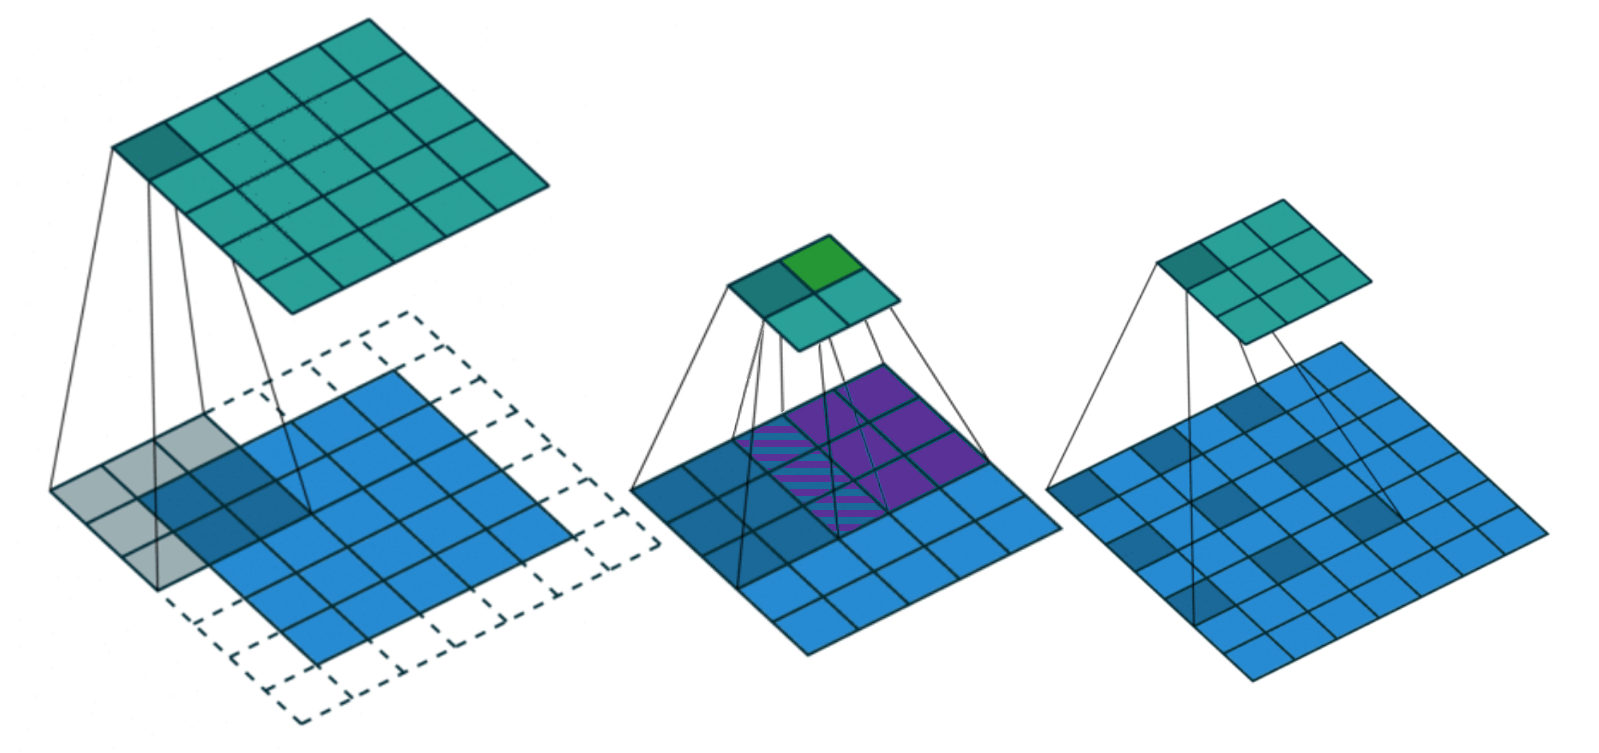
\includegraphics[width=\textwidth]{img/convolutions}
    \caption[Parametrization of convolutional layer]{Effect of padding, stride and dilation on two-dimensional convolutional layer (left to right). Blue maps represent inputs, and cyan maps outputs. Images adopted from \citet{bib:convolution}.}
    \label{fig:convolutions}
\end{figure}

\subsubsection*{Other Layers}
\begin{itemize}
    \item \textbf{Max-pool. k\x k /s P:p} : maximum pooling with kernel size \textit{k\x k}, stride \textit{s} and padding \textit{p}. Default value for stride and padding is 1.
    
    \item \textbf{Fully connected / FC - N} : fully connected layer with \textit{N} neurons
\end{itemize}
\chapter{Application of Neural Networks for Object Detection}
There has been an upsurge in the use of neural networks in recent years. We can partially attribute it to the evolution of hardware allowing for implementation of network models with multiple layers. Deep neural networks (DNNs) are now finding their use in multiple applications in classification, time series prediction, and optimization tasks, and are replacing many older machine learning methods. Some of the benefits of using neural networks include their ability to find and learn complex non-linear relationships in provided data and subsequent generalization to unseen data. However, some applications do not allow for so-called \textit{black box} models and require the reasoning behind the decisions.

Image processing is one of the fields where DNNs are heavily utilized and outperform traditional machine learning approaches with big margins. Uses of DNNs for image processing vary from classification and object detection to auto-encoders for noise removal, and generative networks. A surge in DNN based image processing started in the 2010s with an implementation of a multi-layer convolutional network trained on GPU \cite{bib:deepOnGpu}. 

In this chapter, we take a closer look at how are DNNs applied in object detection. The goal of such a detector is to localize and classify multiple objects of interest in the given image. There are multiple ways of localization, such as semantic segmentation, which categorizes individual pixels, or key-point and skeleton detections. However, we are interested in more straightforward, axis-aligned bounding box predictions. Each of the predicted bounding boxes needs a corresponding class prediction.

Considering the importance of classification in object detection, we dedicate a significant portion of this chapter to describing multiple classification network models. Many detection models directly utilize or are inspired by those classification networks. We also define metrics used to compare the performance of DNN models used for image processing.

\section{Metrics}
In order to evaluate and compare multiple approaches, we require clearly defined metrics. A state-of-the-art model presented without full specification of used evaluation metrics makes comparing multiple such results impossible. Thankfully, there are clearly defined competitions and challenges with precisely defined rules that are often used to make such comparisons. 

The \textit{ImageNet Large Scale Visual Recognition Challenge (ILSVRC)}\footnote{\url{http://www.image-net.org/challenges/LSVRC/}} is most often used to benchmark classification. Object detection is commonly evaluated in two challenges: the \textit{PASCAL Visual Object Classes Challenge}\footnote{\url{http://host.robots.ox.ac.uk/pascal/VOC/}}, and the \textit{COCO Object Detection Task}\footnote{\url{cocodataset.org/}}. Each challenge also provides a public dataset, \textit{ImageNet}, \textit{VOC}, and \textit{COCO} respectively.

In this section, we define metrics used to evaluate those challenges, but also other, not considered qualities. Most notably, none of the challenges mentioned is evaluated based on the speed of the model. Because our work focuses on real-time video analysis, we are interested in finding a balance between accuracy and the number of images processed per second (fps). One more factor to consider would be the physical size of the model, usually represented by the number of parameters and directly impacting the amount of needed memory.

\subsection*{Classification}
The most common and intuitive evaluation metric for classification problems is the number of correctly classified samples as a ratio of all samples. This ratio is referred to as a \textbf{classification accuracy}. However, a complement to the accuracy, \textbf{top-1 error}, is also often used. In \textit{ILSVRC},  alongside top-1 error, a \textbf{top-5 error} is used as another criterion. The top-5 error represents the fraction of test samples in which the correct label does not appear in the top 5 predicted results.

\subsection*{Object detection}
Evaluating a localization and classification of multiple objects in each image is a much complex task than simple classification, mainly because there is no simple one-to-one mapping between ground-truths and predictions. A ground-truth data are a set of \textit{N} boxes with labels, and detector generates a set of \textit{M} boxes with labels and class confidence values.

Because predicted boxes do not perfectly match ground-truths, a matching algorithm is needed to decide whether a prediction is true positive or false positive. Matching is usually done by computing intersection over union (IoU) value for each pair of ground truth and predicted boxes. Then selecting positive detections based on predetermined threshold.
$$\text{IoU} = \frac{\text{Area}(\text{Prediction} \cap \text{Ground truth})}{\text{Area}(\text{Prediction} \cup \text{Ground truth})}$$

With predictions sorted into true positives (TP), false positives (FP) and false negatives (FN) (no predictions matching a ground-truth box) we are able to calculate \textbf{precision} and \textbf{recall}.
$$\text{Precision} = \frac{\text{TP}}{\text{TP}+\text{FP}} = \frac{\text{TP}}{\text{All predictions}}$$
$$\text{Recall} = \frac{\text{TP}}{\text{TP}+\text{FN}} = \frac{\text{TP}}{\text{All ground truths}}$$

With precision and recall defined, we can define the first metrics used for object detection. Note that all following metrics depend on precision and recall, and therefore depend on the IoU threshold.

\subsubsection{Precision-Recall (PR) curve}
For each class, a separate PR curve is plotted. It reveals how much does a change in confidence, influence the precision and recall values. Firstly, predictions for the given class are sorted by a confidence score. For each prediction, precision and recall are then calculated utilizing predictions with a higher confidence score. An object detector of a particular class is considered reliable if its precision stays high while recall increases, which means that predictions with lower confidence score can be considered good predictions.

\subsubsection{Average Precision (AP)}
Comparing curves is not an easy task, particularly if they cross each other frequently, as it often happens with PR curves. However, we can use the area under the PR curve as numerical metrics, called \textbf{average precision}. It is calculated by interpolation, either on all data points or a small number of equally spaced points, \textit{Pascal VOC Challenge} uses 11.

Interpolation equation for all points:
$$\sum_{r=0}^1 (r_{n+1} - r_n ) p_{interp}(r_{n+1})$$
with
$$p_{interp}(r) = \max_{\Tilde{r} \geq r} p(\Tilde{r})$$
where $p(\Tilde{r})$ is precision at recall $\Tilde{r}$.

\subsubsection{Mean Average Precision (mAP)}
Comparing two models class by class is impractical, especially with the classification of hundreds of classes. Therefore, the most often used metrics for object detectors is a \textbf{mean average precision} As the name suggests, it is a mean of AP across the classes. Most common notation, mAP@[0.5] means mAP with IoU threshold 0.5. The mAP can also be averaged over multiple IoU thresholds, mAP@[.5, .95] represents the average mAP from IoU 0.5 to 0.95 usually with step 0.05.

\subsection*{Inference time}
Inference time is a significant factor if we want to consider the model for use in real-time applications. With the state-of-the-art models, images are often processed under a second, often in a few milliseconds. Such small numbers can be hard to visualize. Therefore number of processed \textbf{frames per second} (fps) is more intuitive metrics. However, unlike precision metrics, the fps values are heavily dependant on hardware, software framework, batch size and amount of pre- and post-processing included in the measurement. Hence, only the measurements performed in the identical hardware and software environment can be directly compared.

\section{Classification networks}
\label{sec:clsnets}
A fundamental building block for a modern state-of-the-art classification network is a convolutional layer. Hence, we call this type of networks a convolutional neural networks (CNNs) \cite[ch.~9]{bib:dlbook}. CNN based classifier is a network that given the input image, extracts a feature map from this image and then applies classification layers to produce a confidence score for each possible class. Usually, the soft-max function is applied to the confidence score to get a probability distribution.

We use this section to take a walk through a history of classification CNNs and outline some of the most important models. Some of those models are still used, and others are responsible for inspiring the next generations of even better networks.

\subsection{AlexNet (2012)}
\textit{AlexNet} designed by \citeauthor{bib:alexnet} \cite{bib:alexnet} is the first CNN that won the \textit{ILSVRC} challenge over traditional computer vision and machine learning approaches. It created a foundation on which today's state-of-the-art models are built, and set a new standard for image recognition. \textit{AlexNet's} architecture is a stack of five convolutional layers interleaved by max-pooling layers, and two fully connected layers, followed by a softmax layer. It also popularized the use of ReLU non-linearity in CNNs.

\subsection{VGG (2014)}
\label{sec:VGG}
The network architecture, mostly known as \textit{VGG}, by \citeauthor{bib:vgg} \cite{bib:vgg}, is build onto the deep CNN concept behind \textit{AlexNet}. It managed to prove the feasibility of even deeper network utilizing small convolution filters. 

Each of the \textit{VGG's} convolutional filters employs a 3$\times$3 kernel with the depth of the feature map gradually increasing through the network. In the last layers, the feature map reaches 512 channels. Three fully connected layers and softmax follow the convolutions, see \cref{tab:vggarch}. Multiple versions of the \textit{VGG} architecture can be constructed, depending on the number of convolutional layers. The most popular is the 16 layer version, dubbed \textit{VGG-16}.

The \textit{VGG} network is considered to be a general architecture for a classification network due to its linear architecture with a decreasing area of the features, and an increasing number of channels. 

\begin{table}
    \centering
    \rotatebox{90}{
        \vggArch
    }
    \caption{Architecture of VGG network version D, commonly called VGG-16. Taken from \cite[table 1]{bib:vgg}}
    \label{tab:vggarch}
\end{table}
    
\subsection{Inception (2014)}
\label{sec:inception}
Previous architectures suggests that increasing the number of layers and layer size, leads to better precision. \citeauthor{bib:googlenet} introduced \textit{Inception v1} \cite{bib:googlenet}, also known as \textit{GoogLeNet}, with the goal of increasing precision while improving utilization of computing resources.

Although stacking more convolutional layers increases the accuracy, a growing computational cost of those layers quickly overpowers the benefits. To avoid the aforementioned cost, \textit{Inception} introduces the concept of sparsity in convolutional layers. They achieved sparsity by using \textit{inception modules} that approximate a sparse structure by using multiple convolutions with different kernel sizes and concatenating the outputs together, \cref{fig:incept_mod}. To reduce the computational cost further each convolution is preceded with additional 1$\times$1 convolution, used for a dimensionality reduction. An alternate path in the inception module is provided by max-pooling operation and concatenating it to the output.

\textit{Inception} begins with a sequence of convolution, pooling, and local response normalization operations. This stem is followed by a chain of nine inception modules, ending in a fully connected soft-max classifier. Two auxiliary classifiers are added to intermediate layers of the network to help propagate gradients and provide regularization during the training.

A set of improvements to the \textit{Inception} network is introduced in later versions of the network. Most notably a factorization of convolution layers in Inception v2 and v3, \citeauthor{bib:inception2} \cite{bib:inception2}. Factorization replaces larger convolutions with a network of multiple smaller ones. They found this method very effective, e.g., replacing a 5$\times$5 convolution with two layers of 3$\times$3 results in a relative gain of 28\% and replacing 3$\times$3 layer with 3$\times$1 and subsequent 1$\times$3 layer is 33\% cheaper.

\begin{figure}
    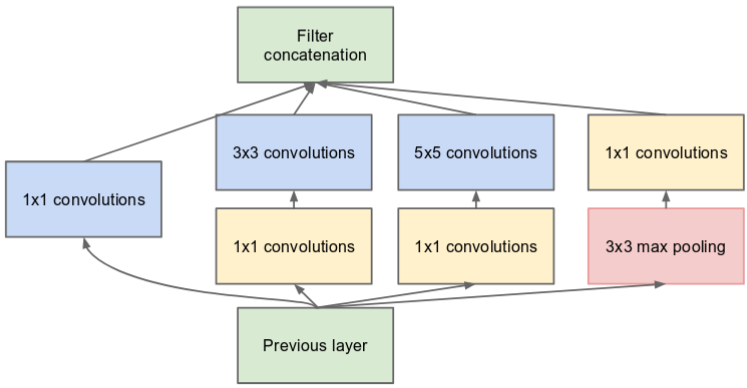
\includegraphics[width=\textwidth]{img/inception}
    \caption{Inception module, picture from \cite[figure 2]{bib:googlenet}.}
    \label{fig:incept_mod}
\end{figure}

\subsection{ResNet (2015)}
\label{sec:resnet}
A trend of adding more layers to CNNs to achieve better accuracy has pushed the limit towards networks with hundred or more layers.  Theoretically, adding more layers to a model should produce equal or better results, based on the fact that shallow model is the subspace of the deeper one. Therefore, additional layers can learn to forward the data. In practice, however, observations suggest that this is not the case, and very deep networks can experience eventual degradation. A solution to this problem was proposed by \citeauthor{bib:resnet} \cite{bib:resnet} in the ResNet architecture, by directly introducing identity functions to the network.

A basic ideas of \textit{ResNet} are directly inspired by the \textit{VGG}. Most of the convolutional layers use 3$\times$3 filters and follow two simple rules: keep the number of filters the same, unless changing the output size and double the filters if the feature size if halved. A newly introduced residual connection bypasses each pair of the convolutional layers and forms a \textit{Basic blocks}. This connection can be an identity function or a 1$\times$1 convolution to match the increased number of filters.

\begin{figure}
    \resnetArch
    \caption{Architecture of the ResNet network and residual blocks. Each of the four \textit{Layers} are created by stacking multiple residual blocks.}
    \label{fig:resnet_arch}
\end{figure}

We can see the high level architecture of this model in \cref{fig:resnet_arch} (left). Each of four \textit{Layers} is a sequence of multiple residual blocks, exact numbers of blocks can be found in \cite[table 1]{bib:resnet}. Previously described \textit{Basic block} with two convolutional layers is used for smaller \textit{ResNet} models (ResNet-18, ResNet-34). Deeper \textit{ResNet} models (ResNet-50, ResNet-101, ResNet-152) use the \textit{Bottleneck block} with three convolutional layers, where the 1$\times$1 layers are responsible for reducing and then restoring dimensions, allowing for a 3$\times$3 layer with a smaller input and output dimensions. Notably, the 152-layer \textit{ResNet} has lower complexity than the 16-layer \textit{VGG} network.



\subsection{Xception (2017)}
\label{sec:xception}
Xception architecture by \citeauthor{bib:xception} \cite{bib:xception}, is heavily inspired by previous architectures, mainly \textit{Inception} and \textit{ResNet}. It is built on the hypothesis claiming: "the mapping of cross-channel correlations and spatial correlations in the feature maps of convolutional neural networks can be entirely decoupled." This hypothesis expands upon the hypothesis underlying \textit{Inception} architectures. Therefore the name \textit{Extreme Inception}. 

The hypothesis is realized in the form of depthwise separable convolution layers. Depthwise separable convolution consists of two steps: a depthwise convolution and pointwise convolution. A depthwise convolution is a convolution performed independently over each channel, i.e., a convolution without changing the number of channels. The second step is a pointwise convolution that uses 1$\times$1 kernel to map the output of depthwise convolution into new channel space.

The architecture is formed by linearly stacking convolutional layers with the addition of residual connections as seen on \cref{fig:xception}. Convolutional layers, non-linearity, and poolings are structured into residual blocks similarly to \textit{ResNet} architecture.

\begin{figure}
    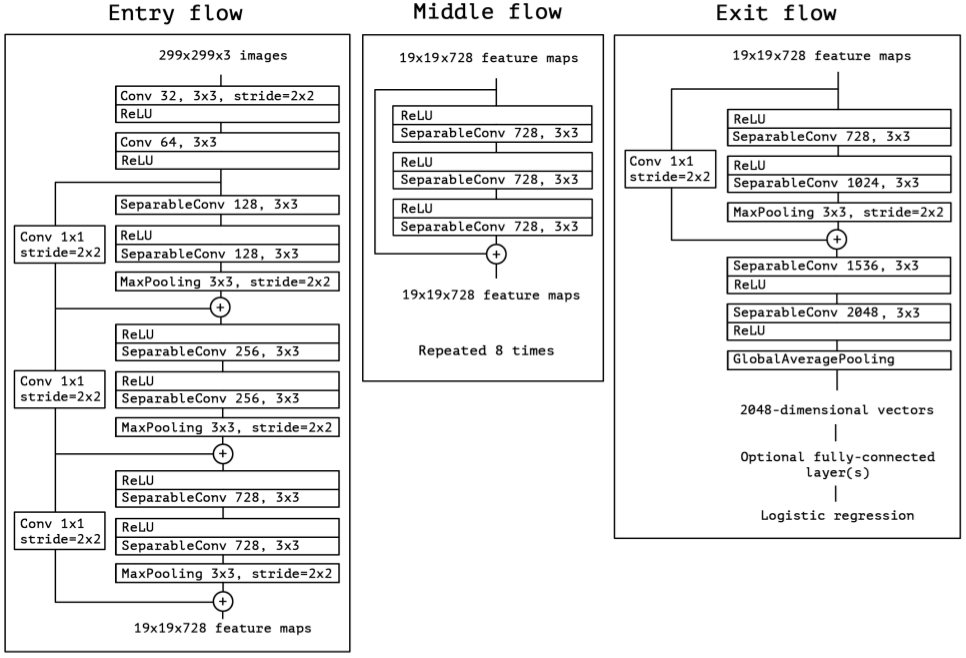
\includegraphics[width=\textwidth]{img/xception}
    \caption{Structure of \textit{Xception} architecture. Taken from \cite[fig. 5]{bib:xception}.}
    \label{fig:xception}
\end{figure}


\subsection{NASNet (2017)}
\label{sec:nasnet}
The difference between this architecture and the others mentioned is that \citeauthor{bib:nasnet} \cite{bib:nasnet} used a machine learning algorithm to design the network. It is a result of a \textit{AutoML}\footnote{\url{https://ai.googleblog.com/2017/05/using-machine-learning-to-explore.html}} project that automates the design of network architecture. Unlike manually designing the network by trial and error, \textit{AutoML} searches space of all possible models, e.g., using reinforcement learning and evolutionary algorithms. The downside of this approach is the computational cost and therefore limitation to small datasets.

\textit{NASNet} is a result of taking an architecture designed for small dataset (\textit{CIFAR-10}\footnote{\url{https://www.cs.toronto.edu/~kriz/cifar.html}}) by \textit{AutoML} and using it to create larger model for \textit{ImageNet} dataset. The model is composed of two types of learned cells, a \textit{Normal Cell} and \textit{Reduction Cell} (see \cref{fig:nasnet}). A general structure of the network is then created by alternating a \textit{Reduction Cell} and \textbf{N} \textit{Normal Cells}

\begin{figure}
    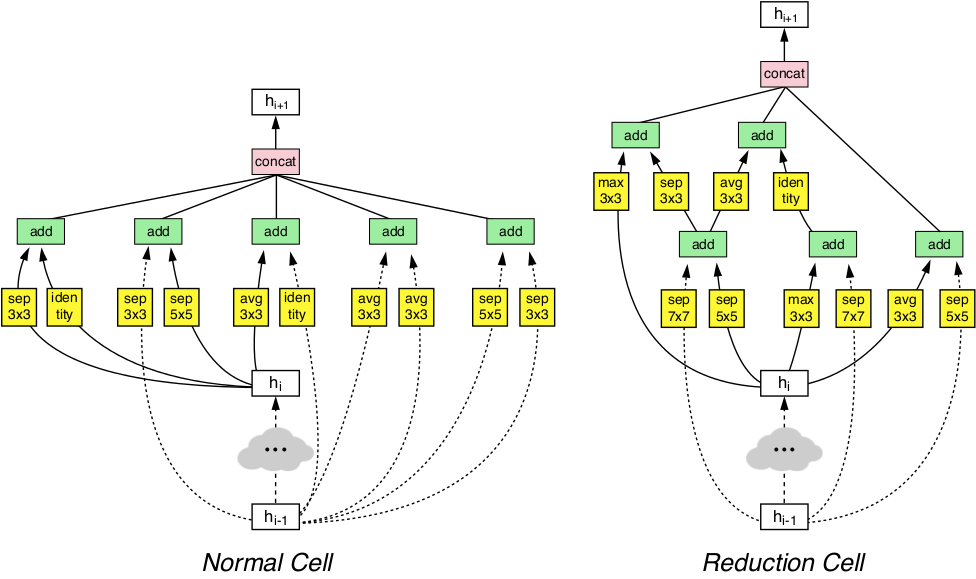
\includegraphics[width=\textwidth]{img/nasnet}
    \caption{Layers used in \textit{NASNet-A}, designed by \textit{AutoML}. Image from \url{ai.googleblog.com/2017/11/automl-for-large-scale-image}.}
    \label{fig:nasnet}
\end{figure}

\subsection{Comparing the classifiers}
At the beginning of this chapter, we mentioned that the classification networks are often compared based on performance on the \textit{ILSVRC} dataset. Newer models, like \textit{Xception}, \textit{NASNet}, and modifications of \textit{ResNet} reach excellent accuracy. However, there is a large discrepancy in their performance considering inference speed. In \cref{fig:cnnbenchmark} we provide an overview of fps-accuracy relationship taken from an independent benchmark by \citeauthor{bib:cnnbenchmark} \cite{bib:cnnbenchmark}. Although the experiment was performed with batch size 1, we expect a universal increase of fps with a bigger batch and only small changes to the relative performance of different models. We can observe a clear trade-off between speed and accuracy for the classification task.

\begin{figure}
    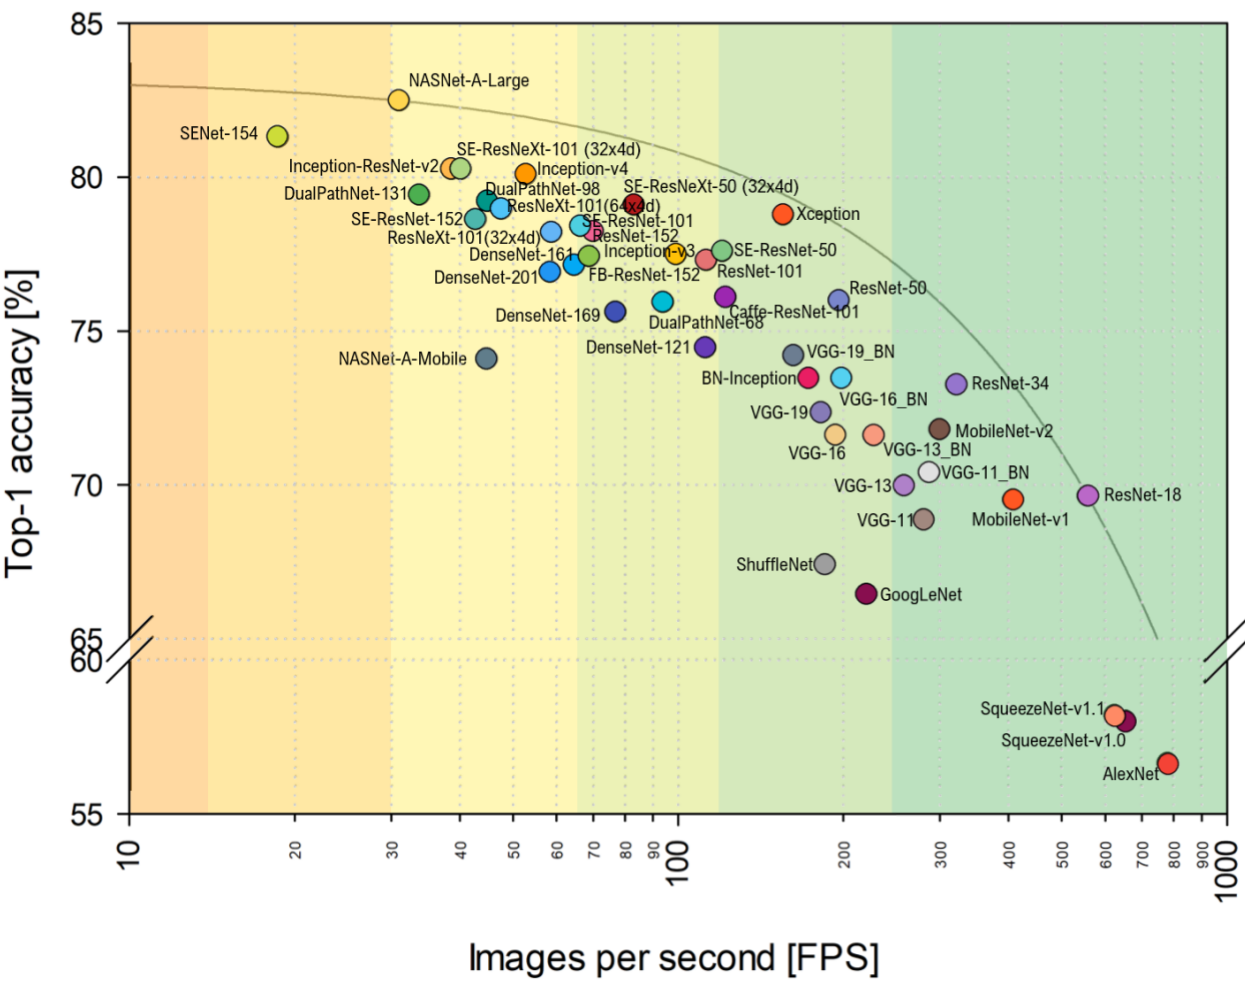
\includegraphics[width=\textwidth]{img/fps_comp}
    \caption{Benchmark of state-of-the-art classification deep neural networks on \textit{ILSVRC} dataset. Performed on NVIDIA
Titan X GPU with batch size 1. Taken from \cite[fig. 3]{bib:cnnbenchmark}}
    \label{fig:cnnbenchmark}
\end{figure}



\section{Detection networks}
\label{sec:detnets}
The goal of object detection is to find and localize all objects of chosen categories. Our focus is on the bounding box (bbox) localization. In this section we describe a family of networks designed for the object detection that all represented state-of-the-art models of their time. Faster R-CNN is still used as one of the best object detectors considering precision. However, inference time is also a important metrics for use in real-time applications, and that is where those models fail. Because this thesis is focused on the real-time application of such networks, we will give entire \cref{chap:rltm} to networks usable for this purpose. 

A training data for detection network consist of set of coordinates and class for each bbox. Expected output for one image is a set of coordinates for bounding boxes, each with an probability distribution of classes. 
\todo{this}

\subsection{R-CNN (2014)}
Region-based Convolutional Network (\textit{R-CNN}) by \citeauthor{bib:rcnn} \cite{bib:rcnn} is the first member of the family of region-based detection models. Each iteration comes with improvements in speed and accuracy. The foundation idea is simple: select regions in the picture and classify each region. This approach leads to a combination of three modules: region proposal algorithm, feature extraction using CNNs on those regions and subsequent classification. 

A naive approach would use a sliding window and classify each cutout of the image. Considering windows for different sizes and aspect ratios of possible objects, this approach would be extremely slow. \textit{R-CNN} solves this problem by applying a region proposal algorithm that selects about 2000 most likely locations of objects. Regions are selected using the \textit{Selective search} \cite{bib:selectivesearch} algorithm and serve as a candidates for bbox predictions. In addition, bounding box regression can be trained to improve bbox prediction accuracy.

Each region is processed separately by a CNN into a feature map. The original architecture uses \textit{Alexnet}, but any classification network can be substituted. Finally, each feature map can be scored. \textit{R-CNN} uses class specific linear support-vector machines instead of a soft-max classification provided by classification CNNs. \Cref{fig:rcnn} illustrates the architecture.

\begin{figure}
    \centering
    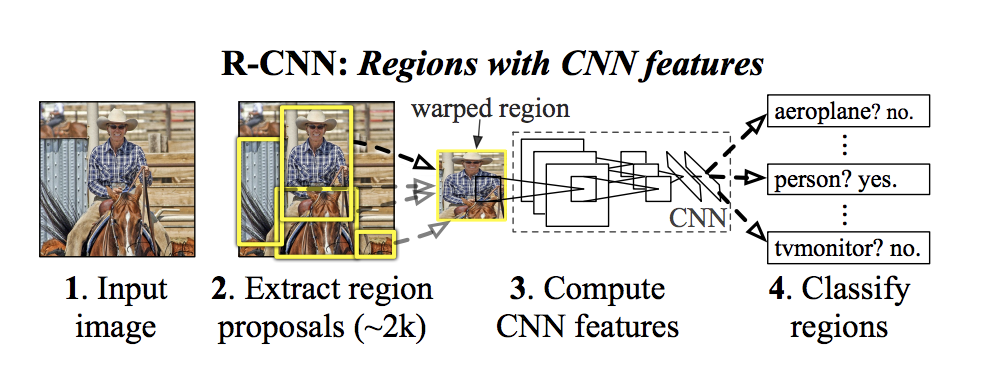
\includegraphics[width=\textwidth]{img/rcnn}
    \caption{R-CNN architecture. Taken from \cite[fig. 1]{bib:rcnn}.}
    \label{fig:rcnn}
\end{figure}

\subsection{Fast R-CNN (2015)}
Even though \textit{R-CNN} was a major step in the right direction, its performance is far from real-time detection. \citeauthor{bib:fastrcnn} \cite{bib:fastrcnn} introduces \textit{Fast R-CNN} with a series of innovations to its predecessor, aimed at improving speed and accuracy. Provided benchmark on the NVIDIA K40 GPU suggests improvements from 47 seconds per image using \textit{R-CNN} with \textit{VGG-16} feature extractor, to 320 milliseconds with \textit{Fast R-CNN} using the same feature extractor, not including a time for SS proposals. 

Similarly to \textit{R-CNN}, this architecture also utilizes region proposal algorithm and a CNN to produce a feature map. A significant drawback of \textit{R-CNN} was computing feature map for each region, despite overlaps. \textit{Fast R-CNN} processes whole input image into a feature map, and then, using a region of interest (RoI) pooling layers, extracts a feature vector for each region. All extracted feature vectors have the same size and are passed through a series of fully connected layers, leading to softmax classifier and bounding box regression layer. An illustration of this process can be seen on \cref{fig:fastrcnn}.

\begin{figure}
    \centering
    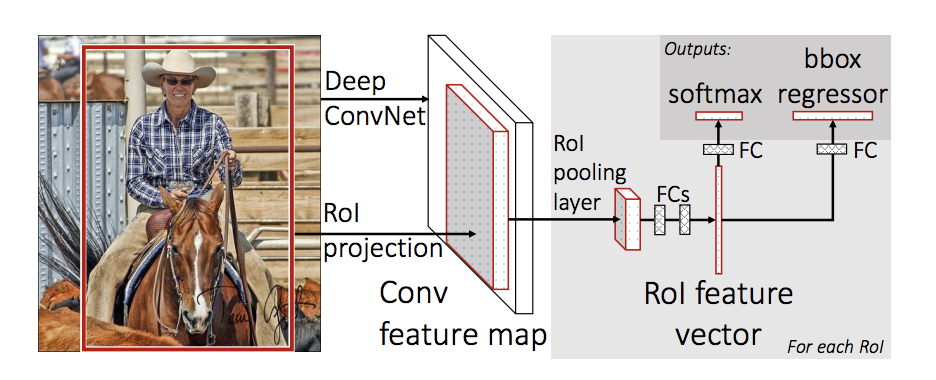
\includegraphics[width=\textwidth]{img/fastrcnn}
    \caption{Fast R-CNN architecture. Taken from \cite[fig. 1]{bib:fastrcnn}}
    \label{fig:fastrcnn}
\end{figure}

\subsection{Faster R-CNN (2015)}
 
 \textit{Faster R-CNN} by \citeauthor{bib:fasterrcnn} \cite{bib:fasterrcnn} expands on the \textit{Fast R-CNN} with the aspiration to achieve a real-time performance. \textit{Fast R-CNN} managed to build a fast feature extraction and subsequent classification usable in a real-time environment but is heavily slowed down by a region proposal SS algorithm. \textit{Faster R-CNN} expands on the idea of sharing resources and replaces selective search with \textbf{region proposal network} (RPN). RPN is built on top of a feature map generated by the feature extractor. As suggested, the feature map is shared between RPN and object detection. This approach is able to achieve 5 fps, which can find a limited use in a real-time environment. Whole architecture can be seen on \cref{fig:fasterrcnn}. 
 
 RPN is designed as a small, sliding-window network, with negligible cost compared to the feature extractor. It is composed of 3$\times$3 convolutional layer with 512 filters and two sibling 1$\times$1 convolutional layers for region regression and classification. Classification in RPNs determines whether proposed region contains an object or a background (\textit{cls} score). Region regression part of the network is tied to the concept of \textbf{anchors}. The anchor is a predefined box centered at a location of sliding-window. Assuming \textit{k} anchors with different sizes and aspect ratios are used, regression produces 4k relative parameters, and classifier 2k scores. Regression parameters are used to modify position and size of their corresponding anchor. The number of regions is then reduced by eliminating proposals with high overlap using a non-maximum suppression (NMS) based on \textit{cls} score. After NMS, top-N ranked proposal regions are used for detection.
 
 To calculate loss and train RPN, a matching between ground-truth boxes and generated region proposals needs to be determined. A positive label is assigned to two kinds of regions: the one with the highest IoU overlap with ground-truth box; regions that have IoU higher than 0.7 with any ground-truth box. A negative label is assigned to a non-positive box if its IoU is lower than 0.3 for all ground-truth boxes. Rest of the boxes do not contribute to training. 
 
 The whole model is trained using a 4-step alternating training:
 
 \begin{enumerate}
     \item train RPN with feature extractor initialized by ImageNet pre-trained model
     \item train separate \textit{Fast R-CNN} using proposals generated by RPN from step 1
     \item train RPN with feature extractor initialized by weights learned by the detector in step 2, fine-tune only layers unique to RPN
     \item using the model from step 3, fine-tune layers unique to \textit{Fast R-CNN}
 \end{enumerate}

Thanks to the modular architecture, \textit{R-CNN} family networks can exploit any CNN as a feature extractor.  Therefore \textit{Faster R-CNN} can achieve state-of-the-art detection results exploiting the latest advances in classification networks and is often used as a benchmark of their performance.
     

 \begin{figure}
     \centering
     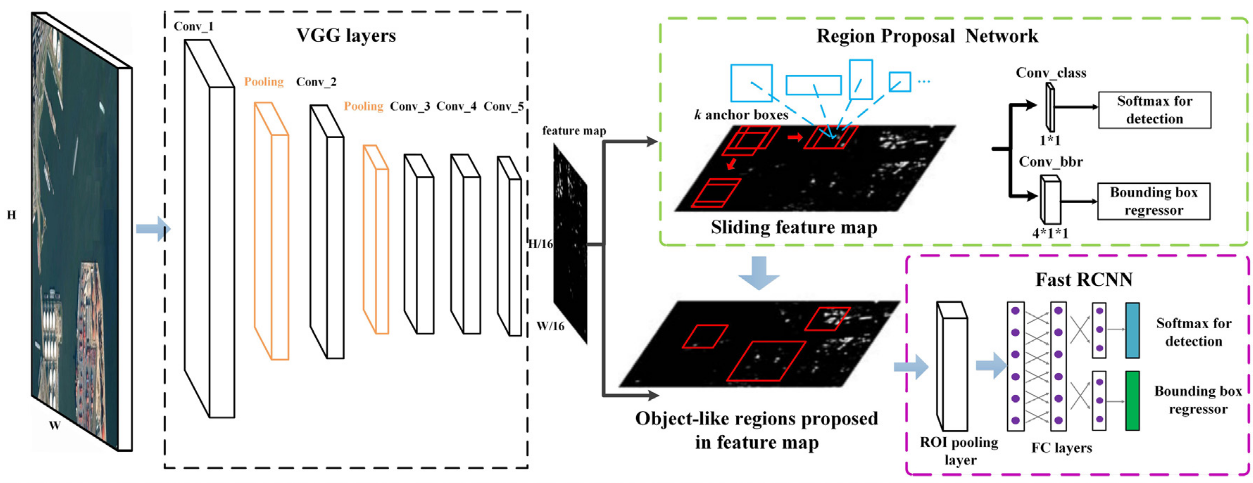
\includegraphics[width=\textwidth]{img/fasterrcnn}
     \caption{The architecture of Faster R-CNN. From \url{https://researchgate.net/figure/The-architecture-of-Faster-R-CNN\_fig2\_324903264}.}
     \label{fig:fasterrcnn}
 \end{figure}

\subsection{Mask R-CNN (2017)}
Previous \textit{R-CNN} based architectures used bounding boxes to localize individual objects. \citeauthor{bib:maskrcnn} \cite{bib:maskrcnn} adds a localization based on semantic segmentation, where the goal is to classify each pixel into a category. \textit{Mask R-CNN} is built upon \textit{Faster R-CNN}, and combines both bounding box localization and semantic segmentation by predicting segmentation masks for each RoI. Product of this approach is a bounding box and class for each object, together with binary segmentation mask. Unlike the semantic segmentation on whole input, applying it on RoIs allows for instantiated segmentation where selected pixels corresponds to given instance of a class.

Implementation and architecture is very similar to \textit{Faster R-CNN}, with two exceptions. One of them is already described, fully convolutional segmentation branch which works in parallel with classification and bounding box regression heads. The other difference is a replacement of RoI pooling layer with RoI alignment layer. The problem of RoI pooling for this purpose is quantization of floating-number RoI to discrete feature map grid and consequent imprecision. RoI align mitigates this problem by using bi-linear interpolation to compute exact values of features at four sampled location in each of RoIs locations and aggregating the results. High level architecture and RoI alignment layer are visualized on \cref{fig:maskrcnn}.

 \begin{figure}
     \centering
     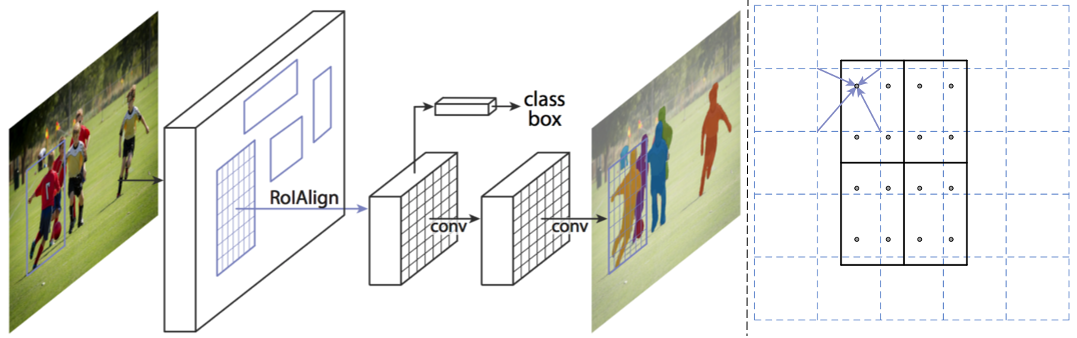
\includegraphics[width=\textwidth]{img/maskrcnn}
     \caption{Left: The architecture of Mask R-CNN. Right: RoI align, grid represents feature map, solid lines an RoI and the dost are the sampling points. From \cite[fig. 1, 3]{bib:maskrcnn}}
     \label{fig:maskrcnn}
 \end{figure}



\chapter{Related Work}
\label{chap:related}

In this chapter, we provide an overview of the methods used for detections in the video. There are two types of approaches that can be used for video detection, a high-speed single frame detector, or a detector designed for a sequence of frames. Although there is no standardized definition of how many fps are real-time, we can consider 25fps as a minimum. However, in practice, we need as much fps as possible not only to keep up with one video stream but to process multiple video streams on one GPU. 

Currently, the detectors designed for image detection hold an edge over detectors with temporal information, mostly because available methods for image detection are faster than temporal methods. However single-frame detectors are unstable and require a lot of post-processing for smooth tracking in video. 

\section{One-Stage Detection}
From our experience, the step from the region-based networks to one-stage detectors can be hard to comprehend. To ease the transition, this section offers a thorough explanation of the one-stage detector building process based on the knowledge of Faster R-CNN network (\cref{sec:fasterrcnn}). 

At this point, we do not concern ourselves with the optimal model but rather present general ideas. We start by defining the input and desired output of such a detector and then explain how to implement it.

\subsection*{Detection Input}
Similarly to Faster R-CNN, we start by processing the input image into a feature map. This process can be done by any feature extraction network, e.g., a classification network up to the fully connected layer. Such a network produces a feature map of [n\x n\x c] size that will serve as a base for our detector.

\subsection*{Desired Output}
To perform a bounding-box detection, we need a parametric representation of both bbox and classification. Since bbox is a rectangle, it can be specified by four parameters: a center position \textit{(X,Y)}, width \textit{W} and height \textit{H}. These values can be either relative in respect to predefined anchor boxes or absolute values.

For a standard soft-max classification, a confidence score for each of the \textit{C} classes is required. However, the network also needs the ability to classify the bbox as a background. An additional parameter with background confidence score \textit{B} can provide the means by being either viewed as a boolean value deciding the presence of an object, or a part of a soft-max classification.

We ended up defining a set of C+5 parameters [c$_1$, ..., c$_C$, B, X, Y, W, H]. In the region-based network, this would represent an output for one region. However, there are no given regions in a one-stage detector, or should we say, every position on a feature map is a region. Given the map [n\x n\x c], we expect to predict described vector of C+5 parameters for [n\x n] cells. This gives us an expected tensor of [n\x n\x C+5] size. 

\subsubsection{Anchor Boxes}
In region proposal networks, we saw the use of multiple anchor boxes. Experiments suggest that it is easier for the network to accept a set of proposed boxes and refine them, rather than regress absolute values by itself. It also helps the generalization if the network can associate boxes with certain aspect rations with certain classes.

There are multiple options to include this feature in our model. For each position, we can either predict \textit{K} anchor box parameters and one set of confidence scores or a separate classification for each box. In the first case, we receive the prediction tensor of [n\x n\x K*4+C+1] shape and in the latter case of [n\x n\x K*(C+5)] shape. For simplification, as the details of the implementation are not necessary, let us call this number of parameters \textit{P}.

\subsection*{Detection}
Now that we know what the input and output of the detector are, we can design the network layers to meet the defined criteria. We will look at both fully connected and convolutional options.

Before we start, however, we feel the need to emphasize, that the detector does not have any information about the purpose of output values. It is designed to generate \textit{P} values for given feature map position, but the information about the association with anchor boxes and classes is provided only during the training process by the correct organization of the ground-truth data and the loss function.

\subsubsection{Fully Connected Detector}
The simplest means of getting from [n\x n\x c] map to [n\x n\x P] values using a fully connected layer is to connect each input value to each output value. It is a functional but clearly a very inefficient solution that requires training of $n^4cP$ parameters. An improvement can be made using an additional fully connected layer with a smaller number of neurons (\textit{b}) and reducing the number of trainable parameters to $n^2b(c+P)$.

Notice that this detector is not only unaware of the order of \textit{P} parameters, but the association of parameters with the feature map position is also not present. A a matter of fact, each predicted parameter is calculated with the information from the entire feature map, and it is only via the training process that the spatial relations are formed.

\begin{figure}
    \centering
    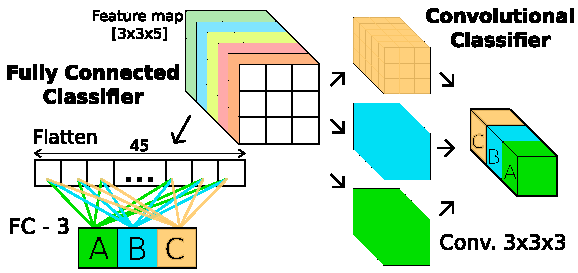
\includegraphics[width=\textwidth]{img/fc_vs_conv}
    \caption[Comparing fully connected and convolutional classifier]{A convolutional layer with kernel size equal to feature map size and no padding performs an equivalent operation as fully connected (FC) layer. While the FC layer is parametrized by the number of neurons and produces the output of size [N], convolution is parametrized by the number of output channels and therefore produces [1\x1\x N] shaped tensor. Kernels are color-coded to match the produced channel.}
    \label{fig:fc_vs_conv}
\end{figure}

\begin{figure}
    \centering
    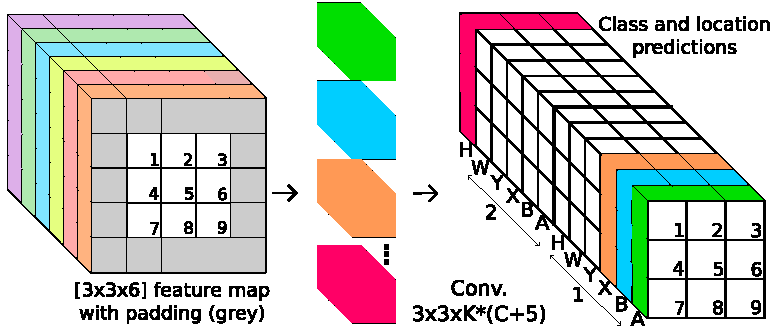
\includegraphics[width=\textwidth]{img/conv_pred}
    \caption[Class and location predictions by convolutional layer]{A single convolutional layer can generate multiple class and location predictions. For every convolutional window it predicts \textit{K = 2} classified bounding boxes. Each prediction composes of four location parameters (height \textit{H}, width \textit{W} and center position \textit{X, Y}), predictions for \textit{C = 1} class  (\textit{A}) and object confidence score (\textit{B}). Kernels of convolution are color-coded to match the produced channel.}
    \label{fig:conv_pred}
\end{figure}

\subsubsection{Convolutional Detector}
Before we start with a convolutional detector, we need to demonstrate the concept by showing the possibility of using a convolutional layer as a classifier equivalent to a fully connected layer. In a classification network with \textit{C} classes, a layer with \textit{C} neurons is connected to the last feature map with [n\x n\x c] shape. This layer takes an input of all $n^2c$ values and outputs a class distribution. On the other hand, let us deploy a convolutional layer with a kernel size of \textit{n\x n} and \textit{C} output channels. From the definition, we know that the actual size of the kernel includes the channel depth equal to the depth of input data and the output number of channels specify the number of such kernels. Now we can see that the application of one convolutional kernel, is in this case equal to one fully connected neuron. The only difference in both approaches is the shape of input and output data. This comparison is illustrated on \cref{fig:fc_vs_conv}.

Now that we know that the convolution can perform the same tasks as a fully connected layer, no matter whether it is classification or regression, we can change the naive fully connected detector to a naive convolutional detector. Of course, this has no benefits other than proving the point.

However, if we decrease the size of the convolutional filter to \textit{k\x k}, where $k < n$, we can use the convolution as a spatially localized detector. The resulting convolutional operation performs detection equivalent to a fully connected detector for each of [n\x n] positions on a feature map, using only local information and producing the \textit{P} parameters for each position. We illustrate the convolutional detector on \cref{fig:conv_pred}.

Thanks to the convolution, we reduced the number of trainable parameters from $n^4cP$ in naive approach to $k^2cP$, where \textit{k} is usually a small number, i.e. \textit{k = 3}, and number of multiplications to $n^2k^2cP$. The other benefit is that convolution performs equivalent detection at each position on the image, where a fully connected detector can acquire some positional biases.



\section{Real-Time Detectors}
\label{sec:rltm}
In \cref{sec:detnets} we took a look on a series of two-stage detectors, with separate region proposals and classification. A few years later, a new type of detectors has been developed, with faster one-stage design. One-stage detectors combine classification and bbox regression into a single pass of the network and are able to achieve real-time performance without problems. Also, the trade-off between speed and precision is continually diminishing in favor of one-stage approach. In this section, we show off two popular approaches \textit{You Only Look Once} and \textit{Single Shot MultiBox Detector}.

\subsection{YOLO: You Only Look Once (2016)}
\label{sec:yolo}
Building on the success of neural network detectors from R-CNN family. \citeauthor{bib:yolo} \cite{bib:yolo} introduced a new approach to object detection. They unify networks for localization and classification into a new single network that predicts both bounding box positions and class probabilities in a single evaluation. This approach also simplifies the training process, as YOLO can be directly trained end-to-end. 

Thanks to straightforward single-pass architecture YOLO claims to perform at 45 frames per second on Titan X GPU. Although it has to sacrifice some precision compared to region proposal methods, it out-performs other real-time systems of its time \cite{bib:overfeat}.


\subsubsection{Detection}
Prediction in YOLO works in a grid-based system. It divides the image into \textit{S\x S} grid with each cell responsible for detecting the object centered in that cell.  Each cell produces predictions for \textit{B} bboxes and one set of class confidence predictions. 

Bbox prediction is composed of four positional parameters and confidence score. Center coordinates relate to the grid cell while width and height are represented relative to the whole image. Confidence score reflects IoU with ground-truth box. Class confidence prediction represents the conditional probability of a said class, given the presence of the object in that cell. 

Final confidence for each box is the product of both conditional class probabilities and the individual box confidence predictions. We can see the illustration of this process on \cref{fig:yoloDet}.

\begin{figure}
    \centering
    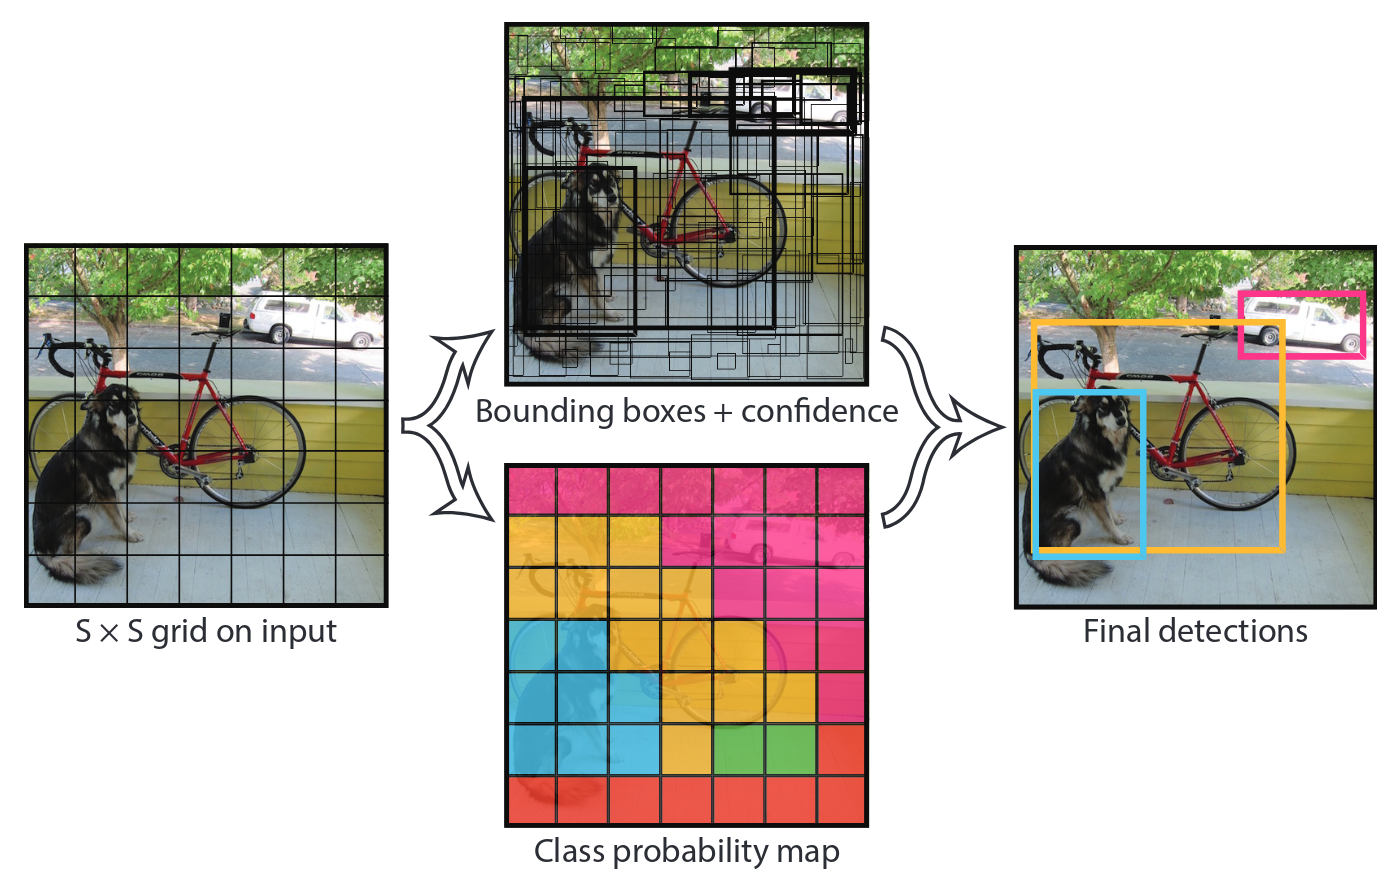
\includegraphics[width=\textwidth]{img/yoloDet}
    \caption[YOLO detection]%
    {Detection process of YOLO. From \cite[fig. 2]{bib:yolo}.}
    \label{fig:yoloDet} 
\end{figure}


\subsubsection{Architecture} 
YOLO is designed as a single network that takes the input image and outputs bbox and class predictions. Design of the network is inspired by Inception classification network. Although it does not use inception modules, it relies on the 1\x1 reduction layers to speed up 3\x3 convolutions. YOLO uses 24 convolutional layers followed by two fully connected layers. Full architecture is shown on \cref{fig:yolo}. 

Various other versions and modifications are possible. A smaller and faster version is called Fast YOLO. It has a similar architecture but uses only 9 convolutional layers. Another possibility to improve YOLO is to replace the custom architecture with a more common feature extractor from a classification network. YOLO build on top of a VGG16 achieves better precision at the cost of half of the frames per second.

\begin{figure}
    \centering
    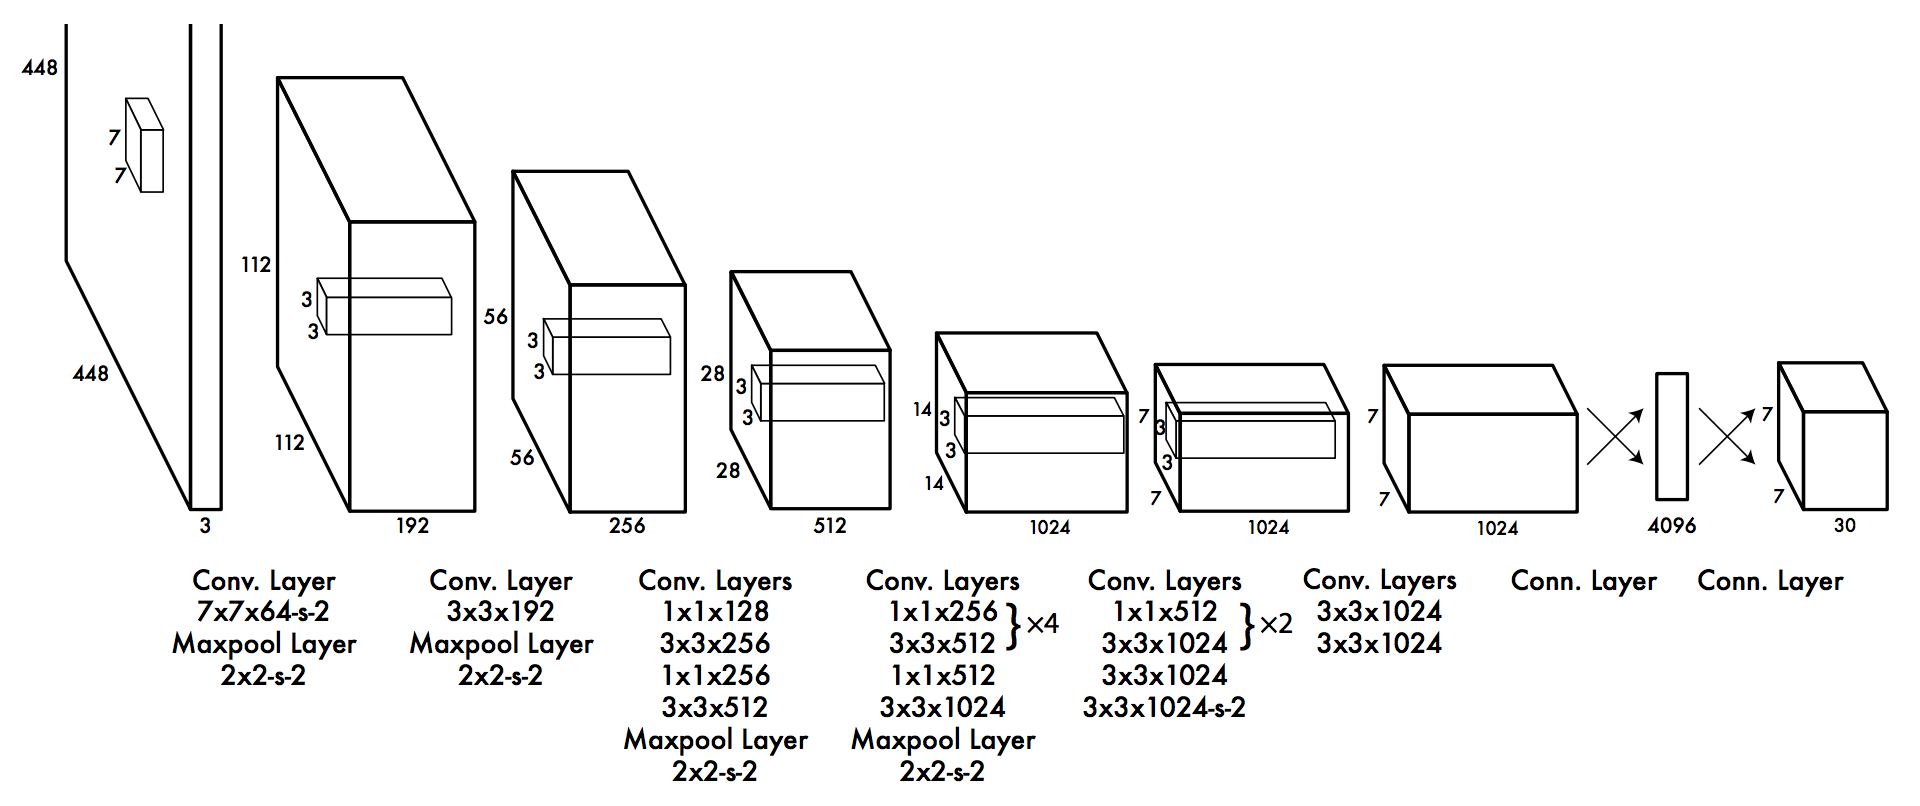
\includegraphics[width=\textwidth]{img/yoylo}
    \caption[YOLO architecture]%
    {YOLO architecture for evaluating PASCAL VOC. It uses 7 by 7 grid with 2 bboxes per cell. Detecting 20 categories, the output's shape is [7\x7\x30]. From \cite[fig. 3]{bib:yolo}.}
    \label{fig:yolo} 
\end{figure}

\subsubsection{Training}
Although the network can be trained end-to-end, it is common for CNN to pre-train on ImageNet dataset. This is also the case for YOLO. First, convolutional layers are pre-trained on the ImageNet dataset, then the detection layers are added, and the whole network is trained for detection. The model is optimized using the sum-squared error between predictions and ground-truths. The loss function is a sum of three parts, classification loss, localization loss, and bbox confidence loss. 

\paragraph{Classification loss}
\begin{align*}
\mathbf{L_{cls}} = \sum_{i=0}^{S^2}\mathbbm{1}_i^{\text{obj}} \sum_{c\in \text{class}} (p_i(c) - \hat{p}_i(c))^2
\end{align*}

\paragraph{Localization loss}
\begin{align*}
\mathbf{L_{loc}} &= \lambda_{\text{coord}} \sum_{i=0}^{S^2} \sum_{j=0}^B \mathbbm{1}_{ij}^{\text{obj}} \left[(x_i - \hat{x}_i)^2 + (y_i - \hat{y}_i)^2\right] \\
 &+  \lambda_{\text{coord}} \sum_{i=0}^{S^2} \sum_{j=0}^B \mathbbm{1}_{ij}^{\text{obj}} \left[(\sqrt{w_i} - \sqrt{\hat{w}_i})^2 + (\sqrt{h_i} - \sqrt{\hat{h}_i)^2}\right]
\end{align*}

\paragraph{Confidence loss}
\begin{align*}
\mathbf{L_{cnf}} &= \sum_{i=0}^{S^2} \sum_{j=0}^B \mathbbm{1}_{ij}^{\text{obj}} (C_i - \hat{C}_i)^2 
+ \lambda_{\text{noobj}} \sum_{i=0}^{S^2} \sum_{j=0}^B \mathbbm{1}_{ij}^{\text{noobj}} (C_i - \hat{C}_i)^2
\end{align*}

\noindent where $\mathbbm{1}^{\text{obj}}_i$ denotes if object appears in cell $i$ and $\mathbbm{1}^{\text{obj}}_{ij}$ denotes that the $j$th bounding box predictor in cell $i$ is responsible for that prediction.

The gradient of cells that do contain the object can be overpowered with the cells that do not.  Therefore, the loss from negative confidence predictions is decreased by $\lambda_{\text{noobj}} = 0.5$. And to emphasize the bbox predictions, localization loss is increased using $\lambda_{\text{coord}} = 5$.In the localization loss, we can see that the center coordinates are handled differently to width and height. The square root of width and height is used to equalize the impact of the absolute value of error in small and large boxes.


\subsubsection{Properties}
A primary virtue of YOLO is its speed for real-time applications, and its simple architecture allows for easy training and end-to-end optimization. YOLO's detection layer is provided with context from the whole image which leads to less false detections than in region proposal methods. 

On the other hand, a significant problem with YOLO's grid-based detection system is a limitation to one class per cell. This limitation results in the inability to detect multiple objects in close proximity, such as people in the crowd. 

YOLO also suffers from multiple problems with precise localization. It learns to detect arbitrary shapes, which can be hard to generalize to objects in new and unusual aspect ratios. Also, it predicts the bboxes on the heavily down-sampled image which leads to further imprecision. 

\subsubsection{YOLO v2 (2017)}
The second version of YOLO architecture by \citeauthor{bib:yolo9000} \cite{bib:yolo9000}, implements a series of improvements to the original network. Compared to original 45fps on [448\x448] image, v2 achieves 59fps on [480\x480] images. 

A selection of changes to YOLO architecture:
\begin{itemize}
    \item \textit{batch normalization} improves precision and helps regularization
    \item \textit{fully convolutional architecture} shortens the inference time
    \item class and confidence predictions are no longer tied to grid locations, instead five \textit{anchor boxes} are used
    \item detection on \textit{multiple feature maps} with different sizes concatenated into channels
    
\end{itemize}


\subsection{SSD: Single Shot MultiBox Detector (2016)}
\label{sec:ssd}
SSD is another real-time detector, aiming to outperform Faster R-CNN by using a single network with one-time evaluation. \citeauthor{bib:ssd} \cite{bib:ssd} presented this model just months after YOLO. Even though these networks are built on similar principles, there are multiple key differences. SSD manages to outperform Faster R-CNN and YOLO both in speed and precision.

\subsubsection{Detection}
One of the main features of SSD is that the detector network is fully convolutional and does not utilize any fully connected layers. Predictions are therefore generated for every position of a convolutional window. SSD adopts similar concept to Faster R-CNN's anchor boxes, this time called default or prior boxes. For each position of the feature map, multiple prior boxes with different aspect ratios are proposed. By default, six boxes are used. Contrary to YOLO, both bbox and classification predictions are made for each position and each prior box.

Bboxes are predicted relative to prior box locations which are themselves relative to a feature map location. \todo{explain} There is no bbox or region confidence value. Instead, SSD uses an additional background class in classification predictions. Considering \textit{B} prior boxes and \textit{C} classes, SSD generates [m\x n\x B\x (C+5)] parameters on feature map of [m\x n] size.

\textit{SSD} detects objects on multiple feature maps at different scales, to accommodate detection of different sized objects. Moreover, this allows detectors on each level to focus on predicting a smaller range of bbox sizes. For the illustration of this process see \cref{fig:ssddet}.

\begin{figure}
    \centering
    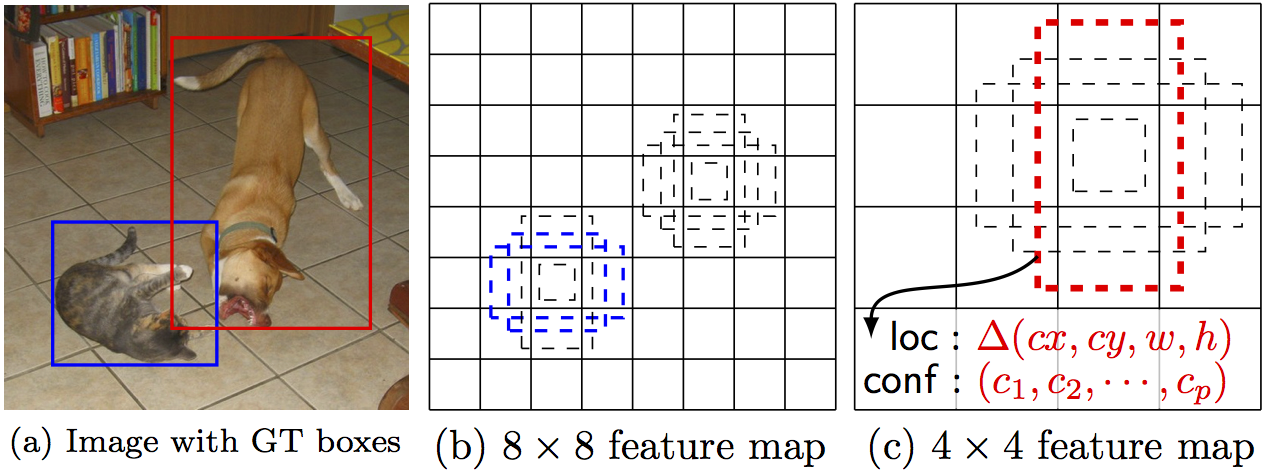
\includegraphics[width=\textwidth]{img/ssddet}
    \caption[SSD detection]%
    {SSD detection. (a) Input image with ground-truth boxes. (b) and (c) Predictions based on prior boxes on multiple scales of feature maps.}
    \label{fig:ssddet}
\end{figure}

\subsubsection{Architecture}
The SSD architecture can be described as a set of three modules. A base network, extra convolutional layers and detection layers.

\begin{itemize}
    \item \textbf{Base network}'s task is to take the input image and produce a feature map. To this end, a feature extractor build from classification network is an ideal candidate. SSD's base is built from VGG16 network with some modifications. First of all, all fully connected layers are removed and replaced with another pair of convolution layers. Pool5 layer is also changed from 2\x2/2 to 3\x3/1 pooling. Technically, SSD does not force any constraints on the base network, and any CNN can replace VGG.
    \item \textbf{Extra layers} serve the purpose of providing more feature maps on decreasing scale to the detector. Smaller feature maps aggregate more information to a smaller area and allow for the detection of larger objects with small convolutional window. On the other hand, information about small objects can be lost. Therefore the use of gradually decreasing series of feature maps. \textit{Extra layers} are implemented as a sequence of convolution layers connected to the end of the \textit{base}.
    \item \textbf{Detection layers} are the final layers of the network. There is a pair of classification and localization convolutions for each feature map. Considering SSD300, where 300 stands for the width and height of input image. Detection is performed on 6 feature maps of sizes [38, 19, 10, 5, 3, 1], using [4, 6, 6, 6, 4, 4] prior boxes respectively, producing 8732 predictions per class. First, two of those feature maps are pulled from the VGG network, and the \textit{extra layers} provide the rest. All detection layers are implemented using 3\x3 convolutions with an appropriate number of filters, as seen on \cref{fig:VGGSSD}.
\end{itemize}

\begin{figure}
    \centering
    \VGGSSD
    \caption[SSD architecture]%
    {SSD architecture based on modified VGG16 network. VGG's three fully connected layers are replaced with two new convolutional layers, and Pool5 layer is changed from 2\x2/2 to 3\x3/1 pooling. Detection on the first and last two feature maps uses four prior boxes, while the rest uses six boxes. See more details on VGG in \cref{sec:VGG}.}
    \label{fig:VGGSSD}
\end{figure}


\subsubsection{Training}
SSD pre-trains the \textit{base network} on ImageNet dataset, and after that removes the classification layers and replaces them with \textit{extra} and \textit{detection} layers. The model is than trained for detection end-to-end. SSD utilizes \textit{smooth L1} loss for localization and \textit{cross-entropy} loss for classification. The final loss is the sum of those two components.

Before the training, we need to figure out which prior boxes match the ground-truth annotations. For each ground-truth box, two criteria are used: a prior box with highest IoU is selected, and then, the ground-truth box is also matched to all prior-boxes with IoU higher than a threshold (0.5). Let the $x_{ij}^p = {0,1}$ be an indicator that $i$th prior box matches $j$th ground-truth box with class $p$.

To keep the balance between positive and negative samples, \textit{hard negative mining} algorithm is employed. Only top negative samples, with the highest confidence score, are chosen. The goal is to keep the ratio of positives and negatives below 1:3.

\paragraph{Localization loss} expresses the error between predicted boxes $(l)$ and ground-truths $(g)$. Predictions are generated in respect to corresponding prior boxes. Therefore, after matching the boxes, a ground-truths also need to be represented in respect to prior box $(d)$, with center $(c_x,c_y)$ and width $(w)$ and height $(h)$.

\begin{align*}
\mathbf{L_{\text{loc}}}(x,l,g) = \sum_{i\in Pos}^N \sum_{m\in(c_x, c_y, w, h)} &x_{ij}^k\text{smooth}_{L1}(l_i^m-\hat{g}_j^m) \\
\hat{g}_j^{c_x} = (g_j^{c_x} - d_i^{c_x}) / d_i^{w} \qquad& \hat{g}_j^{c_y} = (g_j^{c_y} - d_i^{c_y}) / d_i^{h} \\
\hat{g}_j^{w} = log(\frac{g_j^{w}}{d_i^w}) \qquad& \hat{g}_j^{h} = log(\frac{g_j^{h}}{d_i^h})
\end{align*}

\paragraph{Confidence loss} or classification loss, is the softmax loss over class confidences $(c)$.
\begin{align*}
\mathbf{L_{\text{cls}}}(x,c) = -\sum_{i\in Pos}^N x_{ij}^p log(\hat{c}_i^p) - \sum_{i \in Neg} log(\hat{c}_i^0) \quad\text{where} \quad\hat{c}_i^p = \frac{exp(c_i^p)}{\sum_p exp(c_i^p)}
\end{align*}

\paragraph{Total loss} is then a weighted sum of both losses. The weight parameter $\alpha$ is set to 1. The loss is also divided by the number of matched prior boxes to keep it independent of the number of objects.

\begin{align*}
\mathbf{L}(x,c,l,g) = \frac{1}{N}(\mathbf{L_{\text{cls}}}(x,c) + \alpha\mathbf{L_{\text{loc}}}(x,l,g))
\end{align*}

\section{Detection with Temporal Information}
\label{sec:video_det}
In this section, we present two recent models designed specifically for detecting objects in the video. Videos can provide more information to the detector, compared to a set of single independent frames, thanks to the addition of temporal information. Theoretically, using multiple consecutive video frames can provide a large improvement with dealing with detector instability, and occlusions. 

A time-space series of detected bounding boxes is usually referred to as a tube or a tublet. If such a series is generated at once for every object, it can provide smooth tracking and reduce the need for post-processing matching of detections. We use the term chunk to refer to a series of consecutive video frames, to differentiate from the batch of independent images.

However, adding another dimension to the detection model has a performance impact. It is also much harder to create a dataset suitable for training of detectors with a temporal dimension because a whole series of frames need to be precisely annotated. Of course we can find a few public datasets e.g. \textit{ImageNet VID}\footnote{\url{http://image-net.org/challenges/LSVRC/2017/\#vid}}, \textit{YouTube-8M}\footnote{\url{https://research.google.com/youtube8m}} and some smaller ones like \textit{HollywoodHeads}\footnote{\url{https://www.di.ens.fr/willow/research/headdetection}}.

This section presents two approaches to adding temporal information to an object detector. First presented method adopts the approach of region proposal methods and the second one is based on a single-stage detector.


\subsection{Tube-CNN (2018)}
\label{sed:tubecnn}
The architecture of this detector is very similar to Fast-RCNN with the added temporal dimension. The main idea is based on region/tube proposals and the following classification network for those regions. \citeauthor{bib:tubeCNN} \cite{bib:tubeCNN} proved that using a temporal information provided by continuous video frames enhances a precision of the detector. On the other hand, this approach adds more complexity to slower than real-time Faster-RCNN detector. The resulting network achieves only low single digit frame per second values, depending on the configuration. 

\subsubsection{Tube Proposal Network}
Tube proposal generation begins with a feature extraction on a chunk of video frames. After the processing of all frames individually, feature maps are stacked together in the temporal dimension. Then, volumetric convolutional layers (conv3d) are applied to produce a feature volume.

Analogously to Faster-RCNN, each position in this feature volume is used to create tube proposals using \textit{K} anchor tubes. The proposal for each anchor consists of the \textit{objectness} and position parameters. The \textit{objectness} score reflects the probability of the presence of the same objects as opposed to a background. 

IoU value for tubes is defined as a minimum of spatial IoU at the ends of tubes. The number of proposals is reduced by eliminating tubes with high overlap using a non-maximum suppression based on \textit{objectness} score. 

A provided data for the training usually consists of a series of ground-truth boxes for individual frames. During the training of TPN, a series of ground-truth boxes is approximated by a ground-truth tube. Those tubes are then matched against the tube proposals using an IoU threshold. A tube proposal network is designed only to consider tubes corresponding to linear motion in order to limit the complexity. 

\subsubsection{Detection Network}
Tube-CNN, as the name suggests, is a fully convolutional network with the task to extract feature maps from the incoming chunk of images, and using the given tube proposals, classify the tubes and refine the object positions. 

Same as in TPN, the feature extraction is done independently on each frame using some general extractor, e.g., ResNet. Feature maps are then stacked to form a spatio-temporal feature volume. Unfortunately, the provided research paper does not clarify whether the proposal and detection networks share the same extraction layers or not.

A Tube-of-Interest (ToI) pooling is employed on feature volume to select the sub-volume corresponding to each tube proposal. The selected volume is then max-pooled into a fixed-size feature and subsequently used as an input for a classifier. A general convolutional classifier with soft-max activation is used. 

The regression branch of the network predicts the exact position of the object in the first and last frame of the tube. Both regressions begin with RoI pooling on the corresponding feature maps and continue with convolutional layers to produce the positional parameters. 

The detection process is illustrated in \cref{fig:tubecnn}.


\begin{figure}
    \centering
    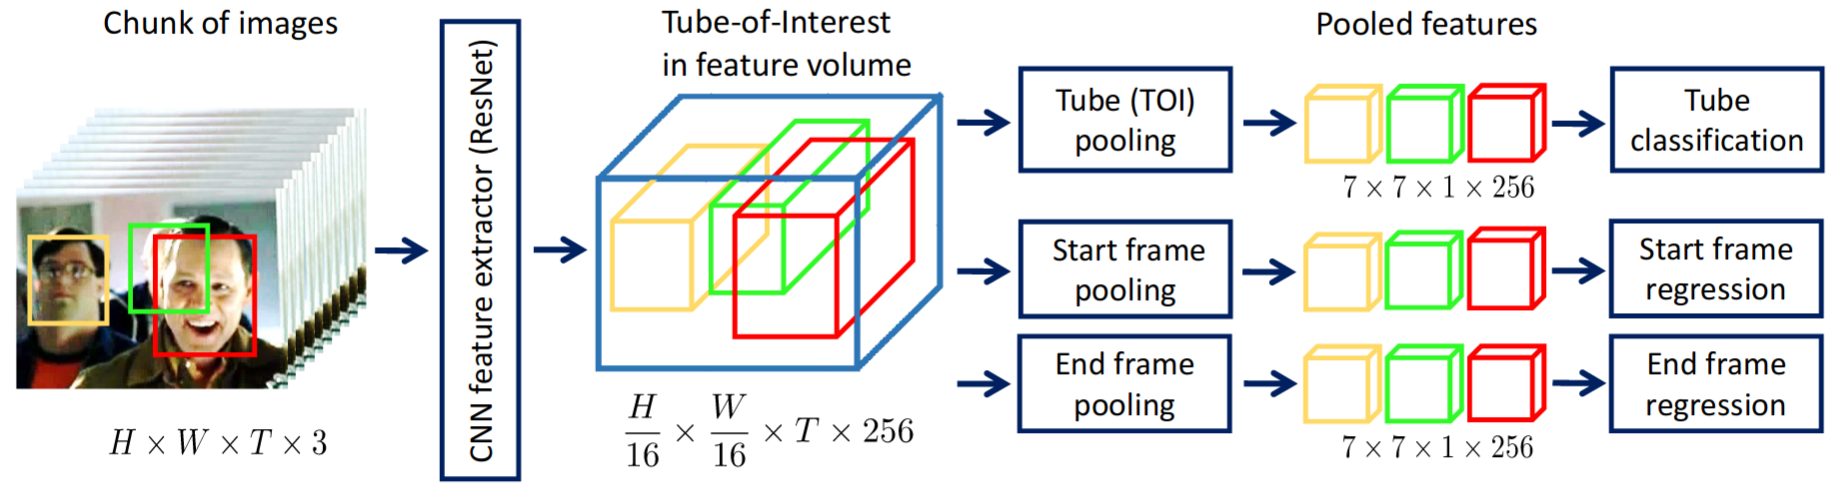
\includegraphics[width=\textwidth]{img/tubecnn}
    \caption[Tube-CNN architecture]%
    {Architecture of Tube-CNN for object detection. Taken from \cite[fig.~2]{bib:tubeCNN}.}
    \label{fig:tubecnn}
\end{figure}


\subsection{TSSD (2019)}
\label{tssd}
\citeauthor{bib:tssd} combine the SSD with recurrent networks \cite[chpt.~10]{bib:dlbook}, namely ConvLSTM cells introduced by \citeauthor{bib:convlstm} \cite{bib:convlstm}, to create a \textit{temporal single-shot detector} (TSSD) \cite{bib:tssd}. They also proposed a tracking module with \textit{Online Tubelet Analysis} working on top of the TSSD.
Compared to SSD's 45fps, TSSD achieves 27fps on ImageNet VID dataset.  

\subsubsection{Architecture}
TSSD is based on a standard backbone of SSD implemented on fully convolutional VGG16 base with extra layers (see \cref{sec:ssd}). This base provides six feature maps that are used for classification and bbox regression in SSD. However, TSSD applies one more layer on the feature maps before detection. This is where the temporal information comes into effect, using the aforementioned convolutional LSTM cells. Two \textit{Attentional ConvLSTM} (AC-LSTM) cells are deployed, one for the bottom three feature maps and one for the top three. Only a small adjustment has been made to the underlying VGG network, that being lowering the number of channels in the second feature map to 512, to equalize the channels in all low-level feature maps. The outputs of both cells are then used for classification and regression in the same way the SSD would do. Details of TSSD implementation, including details on AC-LSTM, can be seen on \cref{fig:tssd}. 

Features contributing to positive object detections are usually unevenly distributed in feature maps and through the scales. Authors proposed the Attentional ConvLSTM cell with the goal of background and scale suppression.  The temporal attention module in AC-LSTM provides the rest of the cell with object-aware features. 

\begin{figure}
    \centering
    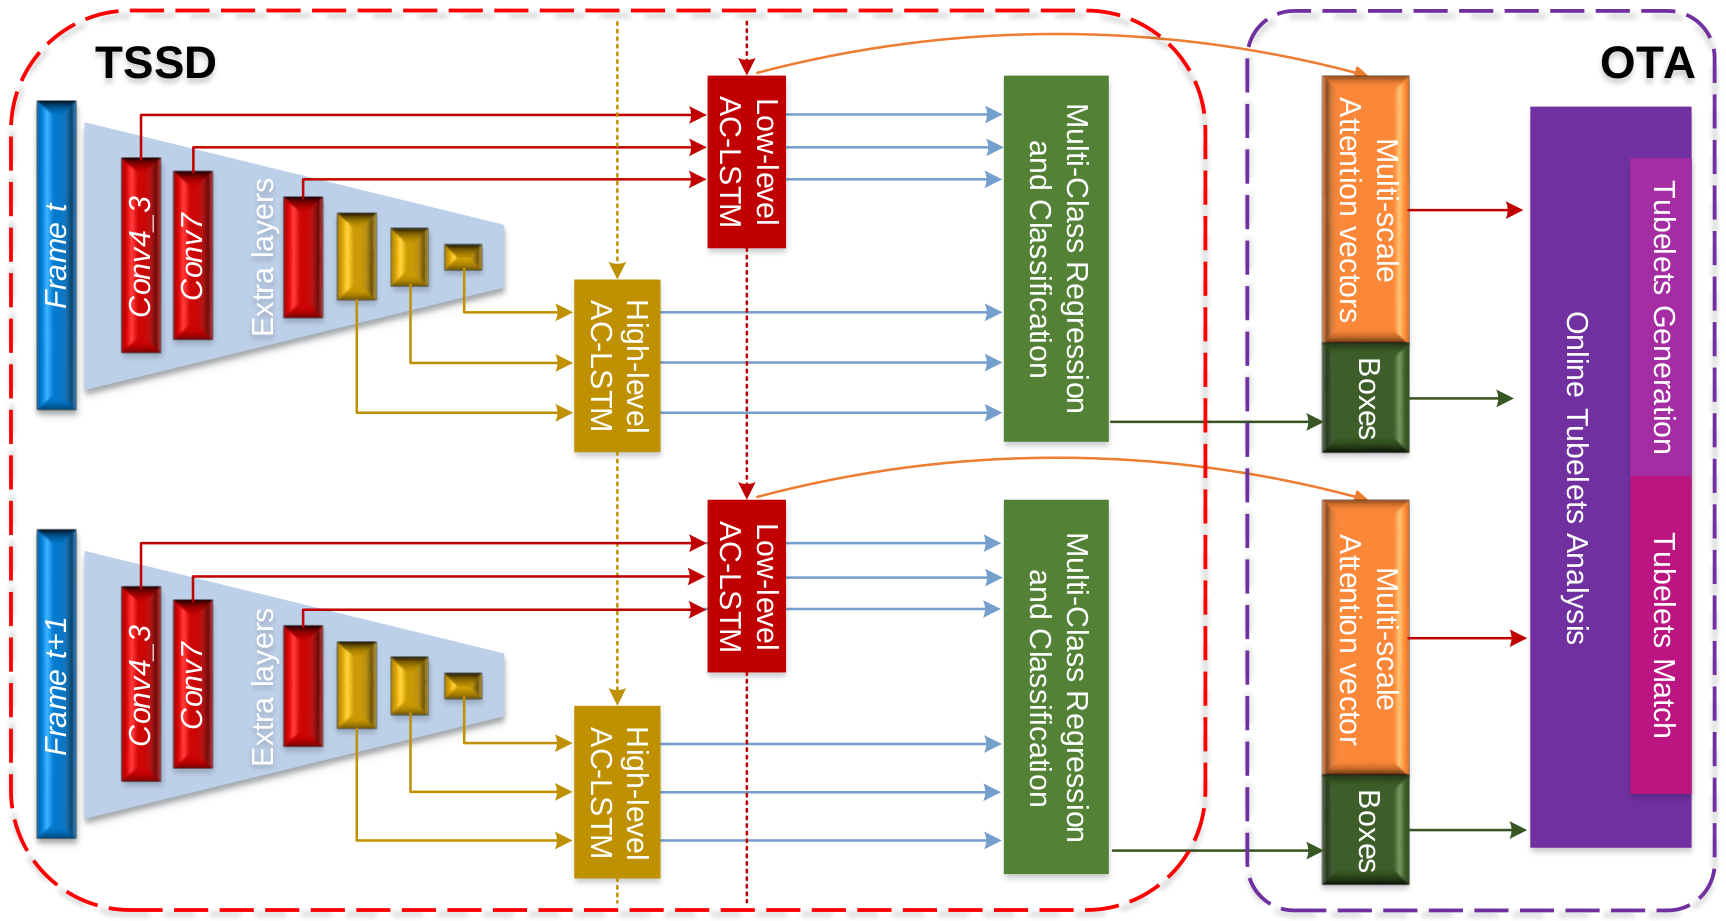
\includegraphics[width=\textwidth]{img/tssd}
    \caption[TSSD architecture and AC-LSTM cell]%
    {Architecture of TSSD (left) and {AC-LSTM} cell (right). \textit{c} denotes concatenation; \textit{Chw-x}, \textit{Elw-x} represent channel-wise and element-wise multiplication, respectively; \textit{+} is element-wise summation. From \cite[fig.~2,~3]{bib:tssd}.}
    \label{fig:tssd}
\end{figure}


\subsubsection{Training}
Similarly to SSD, the loss function of TSSD has multiple objectives weighted by $\alpha, \beta, \gamma$ and $\xi$ constants.

\begin{align*}
\mathbf{L} = \frac{1}{N}(\alpha\mathbf{L_{\text{loc}}} + \beta\mathbf{L_{\text{cls}}}) + \gamma\mathbf{L_{\text{att}}} + \xi\mathbf{L_{\text{asc}}}
\end{align*}


Where $\mathbf{L_{\text{cls}}}$ and $\mathbf{L_{\text{loc}}}$ are defined according to SSD (\cref{sec:ssd}) and \textit{N} is the number of matched boxes.

Attention loss is calculated as a binary cross-entropy loss between ground-truth attention map $A_g$ and prediction maps $A_{_{sc}}$ for each scale $sc$. $A_g$ is a binary map with ones on positions inside ground-truth boxes. Each predicted attention map is up-scaled ($A^{up}_{p_{sc}}$) to match the dimensions of the $A_g$.

\begin{align*}
\mathbf{L_{\text{att}}} = \sum_{sc=1}^6 \mu (-A^{up}_{p_{sc}} log(A_g) - (1-A^{up}_{p_{sc}})log(1-A_g))
\end{align*}

Video frames are generally temporally consistent. Therefore we also expect consistency in detections on short sequences of frames. We can suppress fluctuations in temporal detections by defining association loss. We use class-discriminative score list ($sl$) to represent detection in a frame. $sl$ sums up top-k predictions after application of NMS.

\begin{align*}
\mathbf{L_{\text{asc}}} = (\sum_{t=1}^{seq} sl_t - sl_{avg})/seq
\end{align*}

Where $sl_t$ denotes the score list in frame $t$, $sl_avg$ denotes the average list in a sequence and $seq$ represents the sequence length. 

\chapter{Contributions}

\section{Reimplement SSd on other base}
\subsection{ResNet}
\subsection{NasNet}
pick second net $->$ \cite{bib:benchmark}

\section{Train only specific classes}

\section{something, use video continuity???}
\chapter{Experiments}
\label{chap:exp}

In this chapter, we provide details on the techniques used to gather the data presented in the previous chapter. We also present additional experimental results.


\section{SSD Training}
\citeauthor{bib:ssd} implemented SSD model\footnote{\url{https://github.com/weiliu89/caffe/tree/ssd}} from their research paper using the \textit{Caffe}\footnote{\url{http://caffe.berkeleyvision.org/}} deep learning framework. We decided against performing our experiments in this, by now outdated framework, and implemented our version in newer \textit{PyTorch}\footnote{\url{https://pytorch.org/}} framework (more detailed technical specification of used libraries is available in \cref{app:impl}).

We started by implementing a common framework for SSD detectors, that would support SSD models with many modifications. Although SSDTC inference is possible in the same framework, we had to create a separate environment for the training (more on SSDTC in \cref{sec:ssdtcImpl}). 

The main characteristics of our framework are the use of \textit{SGD} optimizer \cite{bib:sgd} and the loss function defined for SSD, also called MultiBox loss (\cref{sec:ssd}). Another essential element of the detection pipeline, used for inference, is the non-maximum suppression algorithm. The parametrization of these modules can be seen in \cref{tab:trainParams}. It is also worth mentioning that for the sake of consistency, all experimental models were trained for 401 epochs with a batch size of 32, using those default parameters.

\begin{table}
    \centering
    \begin{tabular}{c c|c c| c c}
        \multicolumn{2}{c|}{MultiBox loss} & \multicolumn{2}{c|}{SGD optimizer} & \multicolumn{2}{c}{NMS} \\
        \hline
        IoU threshold & 0.5 & learning rate &  \num{e-3} & IoU threshold & 0.5\\
        \hline
        \multirowcell{2}{positive/negative\\ sample ratio} & \multirowcell{2}{1:3} & \multirowcell{2}{momentum} & \multirowcell{2}{0.9} & \multirowcell{2}{confidence \\ threshold} & \multirowcell{2}{0.2} \\
        & & & & & \\
        \hline
        & & weight decay & \num{5e-4} & & \\
    \end{tabular}
    \caption{A selection of default values for most important parameters in our framework. We used these values for training and evaluation in all experiments. Note that the learning rate decreases during the training.}
    \label{tab:trainParams}
\end{table}


\section{Measurements}
To make our work comparable to other similar studies and future works, we explain methods used for both precision and performance measurements.

\subsection{Precision}
Rather than implementing a copy of the precision evaluation, our precision measurements were taken using an external tool. Using the external tool, independent on our implementation, allows us to easily compare our results with other works with little to no modifications. We used the implementation by \citet{bib:metricsgit} that mirrors the evaluation process of the PASCAL VOC Challenge. The test setup used default parameters, meaning that the interpolation of AP was calculated using all data points and the IoU threshold was set to 0.5. 

We present all the measurements taken on Surveillance dataset while performing multiple experiments described in this thesis in \cref{tab:ap}.


\begin{table}
    \centering
    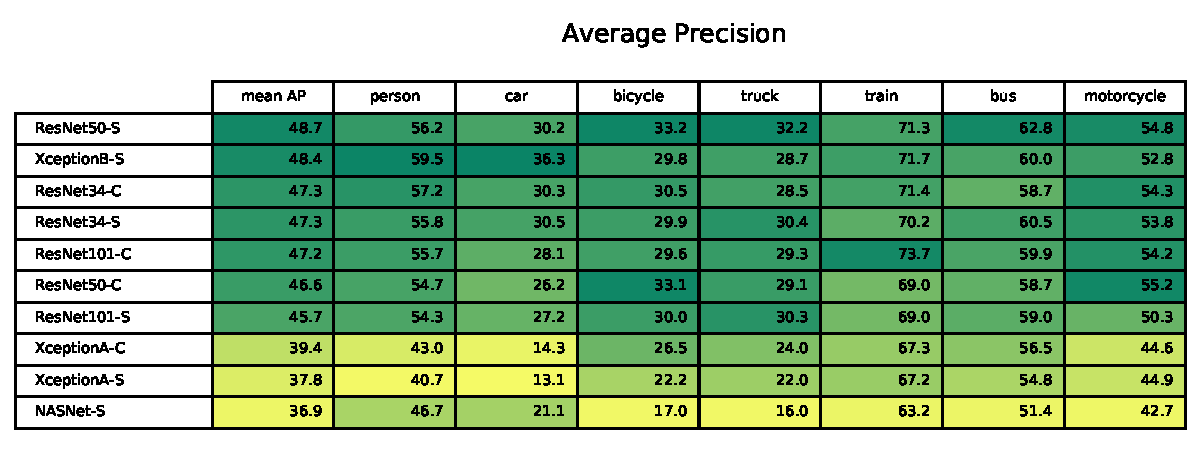
\includegraphics[width=\textwidth]{img/ap}
    \caption[Average precision of all tested networks on Surveillance classes]{Average precision of all tested networks on Surveillance classes. COCO indicates that the network was trained on COCO dataset, otherwise only Surveillance data were used for training.} 
    \label{tab:ap}
\end{table}

\subsection{Inference Speed}
The absolute values of the inference speed measurement would not provide any information without the knowledge of the environment in which they have been taken. In this section, we provide the details of both software and hardware environments used for measurements.

Testing was done by processing a total of 10 000 images in batches of 16. This process was timed, and the average \textit{fps} value was calculated.  Since we do not consider scaling and cropping the images to be part of the network, we did not need to include this process in the measurement. The set of [300\x300] pixel images was pre-loaded into memory before the timer was started. On the other hand, non-maximum suppression is a critical part of the algorithm and is included in the measurement. 

\paragraph{}
\noindent All our testing was done on the following hardware:
\begin{itemize}
    \item AMD EPYC 7401P CPU @ 2GHz \x 24
    \item NVIDIA GeForce GTX 1080 Ti
    \item 128GB DDR4 RAM
\end{itemize}


\section{Improving the Xception-SSD}
In \cref{sec:fixxception} we introduced a hypothesis about Xception\textit{A}-SSD. Based on this hypothesis, we presented the improved Xception\textit{H} model. However, as suggested by the name, it was not our first modification, and we needed some trial-and-error testing to achieve this result.

We will describe every iteration of the Xception-SSD model we trained and the reasoning behind the particular modifications. For clarity, we will refer to the Xception\textit{X} models in this section only by their version letters. The performance of mentioned models on Surveillance dataset is plotted on \cref{fig:xception_perf}, and more details on precision in \cref{tab:ap}. Also, the feature map sizes inside the models are shown in \cref{tab:xmods}.


\begin{figure}
    \centering
    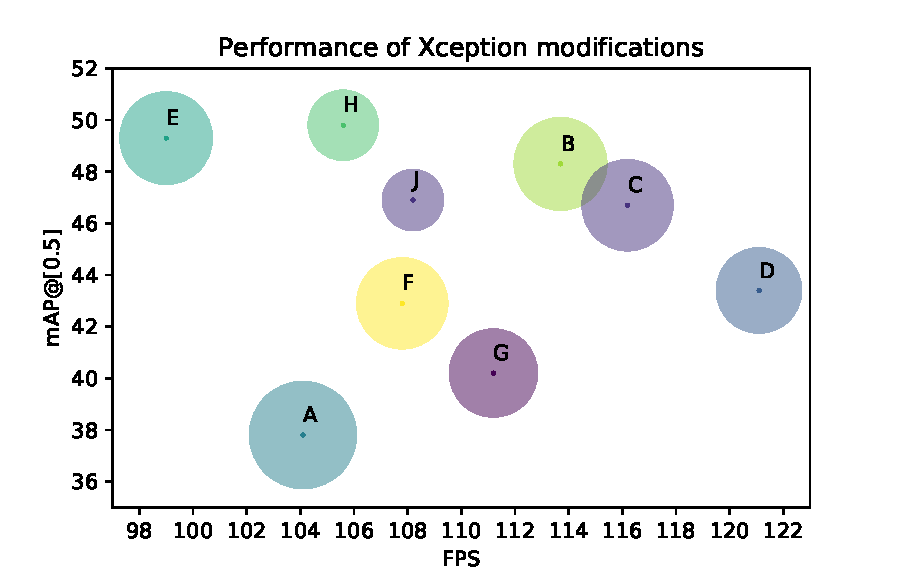
\includegraphics[width=0.95\textwidth]{img/fps_map_x}
    \caption[Performance of multiple Xception modification on Surveillance dataset]{Performance of multiple Xception modification on Surveillance dataset. Circle radii demonstrate relative difference of network parameter counts.} 
    \label{fig:xception_perf}
\end{figure}

\begin{table}
    \centering
    \begin{tabular}{c|c|c|c|c|c}
            &   A   &   B (C, D)   &   E (F, G)   &   H   &   J   \\
        \hline
        B1  &   [74\x128]   &   [74\x128]   &   [74\x128]   &   [74\x128]   &   [74\x128]   \\
        B2  &   \textbf{[37\x256]}   &  [37\x256]   &   [37\x256]   &   [37\x256]   &   [37\x256]   \\
        B3  &   [19\x728]   &   [19\x256]   &   [37\x256]   &   [37\x256]   &   [37\x256] \\
        \hline
        B4-6  &   [19\x728]   &   [19\x256]   &   [37\x256]   &   [37\x256]   &   [37\x256] \\
        B7  &   [19\x728]   &   \textbf{[19\x256]}   &   \textbf{[37\x256]}   &   \textbf{[37\x256]}   &   \textbf{[37\x256]} \\
        B8-10  &   [19\x728]   &   [19\x728]   &   [19\x728]   &   [19\x512]   &   [19\x512]\\
        B11 &   \textbf{[19\x728]}   &   \textbf{[19\x728]}   &   \textbf{[19\x728]}   &   \textbf{[19\x512]}   &   \textbf{[19\x512]}\\
        \hline
        B12 &   [10\x1024]  &   [10\x1024]  &   [10\x1024]  &   [10\x728]  &   [10\x512]\\
        S1  &   [10\x1536]  &   [10\x1536]  &   [10\x1536]  &   [10\x1024]  &   [10\x512]\\
        S2  &   \textbf{[10\x2048]}  &   \textbf{[10\x2048]}  &  \textbf{[10\x2048]}   &  \textbf{[10\x1024]} &  \textbf{[10\x512]}\\
    \end{tabular}
    \caption{A table of feature map sizes on the output of layers of the Xception networks. Bx stand for Xception blocks, S1 and S2 stand for separable convolution layers that follow the block structure (see \cref{fig:xception}). The first number represents spatial dimensions of a square feature, expecting [300\x300] input, and the second one represents the number of channels. The highlighted feature maps are used for the detections. The versions C, D, and F, G share the feature maps sizes with their parent versions, if the given layers are present, but do not match the highlighted feature extraction.}
    \label{tab:xmods}
\end{table}

\subsubsection{Versions B, C, D}
We examine this trio at once,  since version \textit{C} adds modifications to version \textit{B}, and version \textit{D} further modifies version \textit{C}. Notably, we trained these models in parallel and therefore had no results from concurrent models to inform on the design.

Starting with the assumption that the problem of the version \textit{A} is the position of the first feature extraction for detection, we moved the extraction from \textit{block 2} to \textit{block 7}. We also reduced the number of output filters on \textit{blocks 2 to 7} from 728 to 256. As a result, the first detection is performed on a [19\x19\x256] feature map as opposed to the [37\x37\x256] map of \textit{A}. The main factor here, it that the feature map is extracted after the data pass five additional blocks. 

Due to a reduction of feature map size, we considered this modification a half-measure in our plan to move the first feature extraction deeper into the network. However, it proved to be a successful step in the right direction. The network has significantly gained in both speed and precision values. 

Both versions \textit{C} and \textit{D} were designed for observation of the impact of the removal of parts of the network. We designed the modifications in such a way that they would not affect other layers. For clarity, the removals of blocks and layers do not alter the numbering scheme.

Version \textit{C} omits \textit{blocks 5, 6 and 7} and extracts the [19\x19] feature map after \textit{block 10} instead of \textit{block 11}. However, we did not observe a satisfying performance boost to justify received loss of precision. 

Version \textit{D} was designed to test the need for six detection layers, mainly the layers for detecting large objects. It is based on \textit{C} and removes the feature layers produced by \textit{extra layers}. Although the observed performance boost from \textit{C} to \textit{D} was more significant than the one from \textit{B} to \textit{C},  it was also coupled with a major precision penalty.

\subsubsection{Versions E, F, G}
Similarly to the previous trio, these versions are also based on each other, with the main architectural change being applied in \textit{E}. Versions \textit{F} and \textit{G} were designed to perform independent experiments. 

Version \textit{E} is the one, where we finally implemented our original intention of moving the first extracted feature map of [37\x37] size to a deeper layer. Implementation-wise, the only difference between \textit{B} and \textit{E}, is the removal of max-pooling with stride 2 from \textit{block 2} and placing it to \textit{block 8}. This movement results in the increase of feature size to the desired [37\x37] map up to \textit{block 8}.

We observed a noticeable drop-off in performance compared to version \textit{B} and a slight increase in precision. Although the number of parameters in the network is the same, the change from [19\x19] to [37\x37] requires about four times more computation per convolutional layer.

Version \textit{F} modifies \textit{E} in the same way, \textit{C} modified \textit{B}. It skips the \textit{blocks 5, 6 and 7} and extracts the second feature map after \textit{block 10}. Although the received performance boost in relation to \textit{E} is significant, the precision is also significantly impacted in a negative way.

Version \textit{G} repeated the experiment from version \textit{D}, but instead of removing the last three detection feature maps, we removed every other one, thus keeping the first, third and fifth ones. It is based on version \textit{F}, and again we see the precision loss we cannot justify by performance gain.

\subsubsection{Version H}
Since we managed to gain the best precision result with version \textit{E}, we decided to try and increase its performance. To this end, we designed the version \textit{H}. However, tests \textit{C}, \textit{F}, \textit{D} and \textit{G} showed that the removal of blocks or detection layers from the network is detrimental for the result. Therefore we decided for a less radical solution of trimming the channel depth of the network. We ended up trimming the [19\x19] feature map to 512 channels and [10\x10] map to 1024 channels.

Experiments show that this adjustment not only put the performance of the model halfway between \textit{E} and \textit{B} but also slightly boosted the precision.

\subsubsection{Version J}
After the success of version \textit{H}, we decided to try the limits of channel removal approach. We started with the setup of \textit{H}, and set the number of channels of every layer following \textit{block 7} up to \textit{extra layers}, to 512. 

Version \textit{J}, showed us, that this is also not a viable solution. The results are underwhelming in both, precision and performance.


\subsubsection{Conclusion}
In conclusion, we managed to receive the best precision results from the version \textit{H}. Our first implementation, \textit{A}, managed only 37.8\% mAP on Surveillance dataset. Meanwhile version \textit{H} achieved 49.8\% mA on the same data while keeping the performance equivalent.

\section{SSDTC Implementation and Training}
\label{sec:ssdtcImpl}
We have already described the architecture of SSDTC in \cref{sec:ssdtc}; however, the actual implementation and training process proved to be more complicated than SSD. In this section, we go through the challenges brought by SSDTC. 

As mentioned, we based the SSDTC on ResnNet34-SSD. We used the SSD initialized by the weights we learned on Surveillance dataset. We did not need the detection layers of SSD, so we removed them from the model. The resulting ResNet34 with \textit{extra layers} served as a feature extractor for both SSDTC and also for training the baseline SSD on HollywoodHeads dataset. For training of both networks, we froze the weights in the extractor and trained only temporal and detection layers. It is important to note that every image processed by SSDTC, passes through the same extractor. 

The SSDTC design we created, has different input data requirements for training and inference. To properly train, it needs a large number of smallest possible chunks in a batch for the network. However, one large chunk is the most effective way for inference and the most natural way as we expect a continuous video stream.

This, however, poses conflicting requirements for the implementation of the network, namely in the passing of data between the modules. For the purposes of explanation, lets call the ResNet34 network with \textit{extra} layers the \textit{Extractor}, the two conv3d layers the \textit{Temporal module}, and the localization and classification layers the \textit{Detection module}. We will also consider the detection process for only one of six feature map layers of the Extractor. 

During training, the network starts with feature extraction on seemingly independent \textit{n*c} frames in a batch (\textit{c} being the minimal possible chunk, in our case 5, and \textit{n} the batch size). Coming to the temporal layers, the feature maps need to be reshaped to represent \textit{n} chunks of size \textit{c} to allow for conv3d layers. After the temporal layers, the feature maps come out in the batch size of \textit{n}, but due to the nature of temporal layers, the chunk size is reduced to 1. This data then has to be reshaped again, to remove the temporal dimension, and create a batch of size \textit{n} for the detection layers.  

On the other hand, during inference, the input is a single chunk of consecutive frames, that is equivalent to a single batch. This batch can be simply passed thorough feature extraction layers, and the only modification needed for the temporal layers is to encapsulate the whole tensor in additional dimension to represent a temporal batch of size one. After the temporal convolution, we remove the encapsulation and continue with the detection; however, the batch size in this step is smaller than at the beginning. 

We can see the difference between training and inference feature sizes in \cref{tab:ssdtcFeatureSizes}. This behavior forced us into two separate implementations for inference and training. Although both implementations share the same network models, the differences are in the handling of the data between the modules. In the table, we can see that during training, it is the \textit{chunk dimension} that gets eliminated in temporal layers, and during the inference, it is the \textit{batch dimension}. 

Although it is possible to use both versions for training and inference, each has a significant disadvantage if not used as intended. The inference module does not allow for the use of the batch normalization in conv3d layers, because it operates with temporal volume in a batch size one. The fact that the ability to use batch normalization is vital for the training was also experimentally tested. Without normalization, we were not able to over-perform standard SSD with the temporal version. There is a better chance for the training module to be modified for efficient inference, although with some performance hit inherent from our implementation. 

\begin{table}
    \centering
    \begin{tabular}{c|c|c}
        Module &  \multicolumn{2}{c}{Training}\\
        \hline
            & Input   & Output    \\
        Extractor   &  [H$_0$\x W$_0$\x 3\x 5*N] & [H$_1$\x W$_1$\x F$_1$\x 5*N]  \\
        Temporal   &  [H$_1$\x W$_1$\x F$_1$\x 5\x N] & [H$_2$\x W$_2$\x F$_2$\x1\x N] \\
        Detector  &  [H$_2$\x W$_2$\x F$_2$\x N] &      \\
        \hline
        \multicolumn{1}{c}{} & \multicolumn{2}{c}{Inference}\\
         \hline
         & Input   & Output\\
        Extractor   &   [H$_0$\x W$_0$\x 3\x C]  & [H$_1$\x W$_1$\x F$_1$\x C]\\
        Temporal   &  [H$_1$\x W$_1$\x F$_1$\x C\x 1] & [H$_2$\x W$_2$\x F$_2$\x C-4\x 1]\\
        Detector   & [H$_2$\x W$_2$\x F$_2$\x C-4] & \\
        
    \end{tabular}
    \caption{Data shapes and sizes on the input and output of the SSDTC modules. The output of the Detector complies with SSD definitions (\cref{sec:ssd}).}
    \label{tab:ssdtcFeatureSizes}
\end{table}


\chapter*{Conclusion}
\addcontentsline{toc}{chapter}{Conclusion}
This thesis began by briefly summarizing the history of classification networks. We presented a selection of models while describing their architecture and historical significance. With the bases covered, we moved on to the next step towards real-time object detection, region-based networks, and compiled a brief overview of R-CNN family of networks.

Since the focus of this thesis is to optimize the SSD detector for video surveillance, we presented an in-depth examination of this detector. However, it would not be right to present SSD without mentioning its contemporary counterpart, YOLO real-time detection. In order to gain wider knowledge about video detection and get some inspiration for our work, we also examined a pair of video detectors working with temporal information in the video.

From the research paper introducing SSD we know, that the precision of the model can be improved by implementing a sophisticated data augmentation algorithm. Since augmentation algorithms slow down the training process, we decided to start with a fast and straightforward augmentation and focus on the relative comparison of the network performances. We started our work by re-implementing SSD in PyTorch framework and trained in on COCO dataset to serve as our benchmark baseline. 

Our first steps towards optimizing SSD lead to searching for a replacement for the outdated VGG classifier. We tried out ResNet networks, Xception and NASNet. Our finding showed that all tested versions of ResNet were capable of outperforming VGG16, and Xception and NASNet only outperformed VGG in terms of speed. This preliminary result suggested ResNet as a clear choice. However, we were not satisfied with the Xception result and decided to pursue its improvement. 

Before we continued with testing any other architecture modifications, we decided to take a side-step toward the training data. As stated before, our baseline is SSD trained on COCO dataset. However, we are not interested in every class contained in COCO. As a matter of fact, we are only interested in seven of those eighty classes. Before jumping straight to training with only those selected classes, we formulated the hypothesis, according to which the precision of the detector can be negatively impacted by the removal of the unwanted classes from the training process. We performed two tests concerning limiting the number of detected classes, one experiment to test our hypothesis and therefore precision, and second test to observe the relationship between the number of detected classes and speed of the network. The performance test was inconclusive and did not favor one dataset over the other. However, the inference speed test clearly shows the benefits of a lower number of classes. With ResNet50-SSD, we managed to speed up the network from 50 fps on 80 classes to 123 fps on 7 classes. Based on the results of those tests, we decided to continue with all further experiments with this limited dataset.

With training dataset taken care of, we returned to the Xception-SSD and its disappointing precision. As it usually goes with neural networks, we took an experimental approach and designed multiple versions of Xception to test. After a few iterations, we arrived at the Xception version H, that met our expectations. This version managed to perform on par with ResNet50-SSD, reaching over 49\% mAP on surveillance data, however still under-performing it in terms of speed. 



\section{Future Work}






%%% Bibliography
%%% Bibliography (literature used as a source)
%%%
%%% We employ bibTeX to construct the bibliography. It processes
%%% citations in the text (e.g., the \cite{...} macro) and looks up
%%% relevant entries in the bibliography.bib file.
%%%
%%% The \bibliographystyle command selects, which style will be used
%%% for references from the text. The argument in curly brackets is
%%% the name of the corresponding style file (*.bst). Both styles
%%% mentioned in this template are included in LaTeX distributions.

%\bibliographystyle{plain}    %% Author (year)
%\bibliographystyle{unsrt}     %% [number]

\renewcommand{\bibname}{Bibliography}

%%% Generate the bibliography. Beware that if you cited no works,
%%% the empty list will be omitted completely.

\bibliography{bibliography}

%%% If case you prefer to write the bibliography manually (without bibTeX),
%%% you can use the following. Please follow the ISO 690 standard and
%%% citation conventions of your field of research.

% \begin{thebibliography}{99}
%
% \bibitem{lamport94}
%   {\sc Lamport,} Leslie.
%   \emph{\LaTeX: A Document Preparation System}.
%   2nd edition.
%   Massachusetts: Addison Wesley, 1994.
%   ISBN 0-201-52983-1.
%
% \end{thebibliography}


\appendix
\chapter{Implementation of SSD}

% \todo{implement app that takes video and outputs annotations in standardized format}

% \todo{implement viewer: video+annotations->stream}




%%% Figures used in the thesis (consider if this is needed)
%\listoffigures
% list of figures je dobrej do knizek co maj 500+ stranek, tady to je uplna zbytecnost.

%%% Tables used in the thesis (consider if this is needed)
%%% In mathematical theses, it could be better to move the list of tables to the beginning of the thesis.
%%%\listoftables

%%% Abbreviations used in the thesis, if any, including their explanation
%%% In mathematical theses, it could be better to move the list of abbreviations to the beginning of the thesis.
%%%\chapwithtoc{List of Abbreviations}

%%% Attachments to the bachelor thesis, if any. Each attachment must be
%%% referred to at least once from the text of the thesis. Attachments
%%% are numbered.
%%%
%%% The printed version should preferably contain attachments, which can be
%%% read (additional tables and charts, supplementary text, examples of
%%% program output, etc.). The electronic version is more suited for attachments
%%% which will likely be used in an electronic form rather than read (program
%%% source code, data files, interactive charts, etc.). Electronic attachments
%%% should be uploaded to SIS and optionally also included in the thesis on a~CD/DVD.
%%% Allowed file formats are specified in provision of the rector no. 23/2016.
%\chapwithtoc{Attachments}

\openright
\end{document}
